\documentclass[10pt,twocolumn,letterpaper]{article}

\usepackage{cvpr}
\usepackage{times}
\usepackage{epsfig}
\usepackage{graphicx}
\usepackage{amsmath}
\usepackage{amssymb}
\usepackage{bbm}
\usepackage{mathtools}

\usepackage[utf8]{inputenc}
\usepackage[english]{babel}
\usepackage[T1]{fontenc}

\usepackage{subcaption}
\usepackage[draft,inline,nomargin]{fixme} % Enable fixme-notes.
\usepackage{units}

\usepackage{multicol}

\makeatletter
\newcommand*\rel@kern[1]{\kern#1\dimexpr\macc@kerna}
\newcommand*\widebar[1]{%
  \begingroup
  \def\mathaccent##1##2{%
    \rel@kern{0.8}%
    \overline{\rel@kern{-0.8}\macc@nucleus\rel@kern{0.2}}%
    \rel@kern{-0.2}%
  }%
  \macc@depth\@ne
  \let\math@bgroup\@empty \let\math@egroup\macc@set@skewchar
  \mathsurround\z@ \frozen@everymath{\mathgroup\macc@group\relax}%
  \macc@set@skewchar\relax
  \let\mathaccentV\macc@nested@a
  \macc@nested@a\relax111{#1}%
  \endgroup
}
\makeatother

\graphicspath{{pictures/}}

% Include other packages here, before hyperref.

% If you comment hyperref and then uncomment it, you should delete
% egpaper.aux before re-running latex.  (Or just hit 'q' on the first latex
% run, let it finish, and you should be clear).
\usepackage[pagebackref=true,breaklinks=true,letterpaper=true,colorlinks,bookmarks=false]{hyperref}

%\cvprfinalcopy % *** Uncomment this line for the final submission

\def\cvprPaperID{****} % *** Enter the CVPR Paper ID here
\def\httilde{\mbox{\tt\raisebox{-.5ex}{\symbol{126}}}}

% Pages are numbered in submission mode, and unnumbered in camera-ready
\ifcvprfinal\pagestyle{empty}\fi
\begin{document}

%%%%%%%%% TITLE
\title{Tri-modal Human Body Segmentation}

\author{Chris Bahnsen, Andreas Møgelmose, Thomas B. Moeslund\\
Aalborg University\\
Sofiendalsvej 11, 9200 Aalborg SV, Denmark\\
{\tt\small \{cb, am, tbm\}@create.aau.dk}
% For a paper whose authors are all at the same institution,
% omit the following lines up until the closing ``}''.
% Additional authors and addresses can be added with ``\and'',
% just like the second author.
% To save space, use either the email address or home page, not both
}

\maketitle
%\thispagestyle{empty}

%%%%%%%%% ABSTRACT
\begin{abstract}
   The ABSTRACT is to be in fully-justified italicized text, at the top
   of the left-hand column, below the author and affiliation
   information. Use the word ``Abstract'' as the title, in 12-point
   Times, boldface type, centered relative to the column, initially
   capitalized. The abstract is to be in 10-point, single-spaced type.
   Leave two blank lines after the Abstract, then begin the main text.
   Look at previous CVPR abstracts to get a feel for style and length.
\end{abstract}

%%%%%%%%% BODY TEXT
\section{Introduction}
\label{sec:introduction}

Segmentation of people in images is still nowadays a very challenging and tough problem for the computer vision community due to the great diversity of poses that they can adopt and their variable appearance. Difficulties also arise from changes in lighting conditions and complex and cluttered backgrounds. The general idea of human body segmentation is to assign a label to every pixel or group of pixels in an image such that pixels with the same label share certain visual characteristics which entitles them to be considered as part of a human. These type of problems are commonly referred to as labeling problems. Despite extensive research done so far, some constraints have still to be taken into account and one often has to make assumptions about the scenario where the segmentation task is to be applied, such as static versus moving camera, indoor versus outdoor, and so on. Ideally, it should be tackled in an automatic fashion rather than relying on user intervention, which makes such task even more challenging. 

There exist a wide range of possible applications for people segmentation such as surveillance, content-based image retrieval, activity recognition, patient caregiving, or human-computer interaction among others. Such task is also often related to pose estimation problems, since it can be carried out efficiently once the person is detected and segmented in an image. Furthermore, it can facilitate the task of photo edition, chroma-keying, or video compression. Hence, human body segmentation can be considered as an important preprocessing step for other tasks.

State-of-the-art methods that tackle the human segmentation task mostly use color images recorded by RGB cameras as the main cue for further analysis, although they present several widely known intrinsic problems such as intensity similarities between background and foreground. More recently, the release of RGB-Depth devices such as Microsoft\textsuperscript\textregistered Kinect\textsuperscript\texttrademark , a cheap multi-sensor device based on structured light technology, has allowed the community to use RGB images along with per-pixel depth information, often called depth maps, thus increasing the robustness of the methods. Besides, this device has helped boost research in human pose and behavior analysis.

In this context, we propose adding a third modality: thermal imagery got from thermal infrared cameras, thus complementing other information sources and making easier the segmentation task. Although thermal cameras are relatively expensive devices, their market price is lowering substantially every year -- as it happens with other sensory devices. Moreover, they can capture data similar to standard color cameras but without having illumination problems, that is why infrared cameras are becoming popular in surveillance scenarios and other similar applications. 

In this context, we introduce a novel tri-modal dataset that contains people acting in three different video sequences -- consisting of more than 10,000 frames in total -- recorded with a fixed multi-sensory device setup, consisting of a Microsoft\textsuperscript\textregistered Kinect\textsuperscript\texttrademark and a thermal camera. In them, three different people appear concurrently in two different indoor scenarios, performing diverse actions that involve interaction with objects, such as reading, working with a laptop, speaking on the phone, and so on and so forth. The dataset is presented along with an algorithm that performs the calibration and registration among modalities. In addition, we propose a baseline methodology to automatically segment people appearing in the video sequences. Firstly, color and depth cues are registered using intrinsic parameters of the Kinect\textsuperscript\texttrademark device, whereas thermal is registered to color at nearly pixel-level. Secondly, we learn a model of the background using the initial set of depth frames of each sequence to subsequently perform background subtraction, segmenting subject candidate regions. Having candidate regions segmented in all the available and registered modalities, they are described using simple but reliable feature uni-modal feature descriptors. Then, the descriptions are used to learn probabilistic models (e.g. Gaussian Mixture Models) so as to predict the candidate regions actually belonging to people. The predictions got from different models are subsequently fused using both heuristic and learning-based approaches. We will compare results from applying segmentation to the different modalities separately to results obtained by fusing features from all modalities. To the best of our knowledge, this is the first dataset and work that combines color, depth and thermal modalities to perform the people segmentation task in videos, aiming to bring further benefits towards developing more robust solutions.

The rest of this paper is organized as follows: Section~\ref{sec:relatedwork} reviews the different approaches for human body segmentation that appear in the recent literature. Section~\ref{sec:setup} explains the acquisition and multi-modal calibration process, whereas Section~\ref{sec:registration} describes the registration algorithm between modalities. Section~\ref{sec:trimodalhumanbodysegmentation} introduces and exhaustively explains the proposed baseline methodology, which will be experimentally evaluated in Section~\ref{sec:evaluation} along with the registration algorithm. Finally, Section~\ref{sec:conclusions} concludes the paper.

\section{Related work}
\label{sec:relatedwork}

Within the last decade a great number of novel approaches have emerged to respond to different requirements in the human segmentation context, such as trying to overcome changing illumination conditions, dealing with variable human poses or developing quasi-automatic systems that progressively lose the need for user intervention.
 
 When dealing with indoor scenarios recorded by a stationary camera, the pixel-based background subtraction approach can be applied successfully. We can model the background distribution of the scene and detect moving objects by comparing each pixel to the model, which are considered as foreground. The result is a silhouette of the moving object, which can be further used for other tasks. Pixel intensity is the most commonly used feature in background modeling, though there are many approaches that use other type of information such as edge, motion, stereo or texture features. The parametric model that Stauffer and Grimson proposed in \cite{stauffer1999adaptive}, which models the background using a mixture of gaussians (MoG), has been widely used and many variations have been suggested based on it. In \cite{bouwmans2011recent}, more advanced statistical background modeling techniques are deeply reviewed. 
 
Nonetheless, after obtaining the moving object contours we still need a way to assess whether they belong to a human or not. Human detection methods are strongly related to the task of human body segmentation since they allow to discriminate better between other objects. They usually produce a bounding box indicating where the person is, which in turn may be also useful as a prior for pixel-based or bottom-up approaches to refine the final human body silhouette. In the category of holistic body detectors, one of the most successful representations is the Histogram of Oriented Gradients (HOG) \cite{dalal2005histograms}, still being the basis of many current detectors. Used along with a discriminative classifier --e.g. Support Vector Machines (SVM) \cite{hearst1998support} --it is able to accurately predict the presence of human subjects. Example-based methods \cite{andriluka2010monocular} have been also proposed to address human detection, utilizing templates to compare the incoming image and locate the person, limiting the pose variability though.  

Regarding descriptors, other possible representations apart from the already commented HOG are those that try to fit the human body into silhouettes \cite{mittal2003human}, those that model color or texture such as Haar-like wavelets \cite{viola2005detecting}, optical flow quantized in Histrograms of Optical Flow (HOOF) \cite{dalal2006human}, depth maps \cite{plagemann2010real} and, more recently, descriptors including logical relations, e.g. Grouplets \cite{yao2010grouplet}, which enables to recognize human-object interactions.

Instead of whole body detection, some approaches have been built under the assumption that the human body consists of an ensemble of body parts \cite{ramanan2006learning, pirsiavash2012steerable}. Some of them are based on pictorial structures \cite{andriluka2009pictorial, yang2011articulated}. In particular, \cite{yang2011articulated, yang2012articulated} from Yang and Ramanan along with \cite{felzenszwalb2010object} from Felzenszwalb have outperformed other existing methods using a Deformable Part-based Model (DPM) that consists on a root HOG-like filter and different part-filters that define a score map of an object hyphotesis, using latent SVM as a classifier. Another well-known part-based detector is Poselets \cite{bourdev2009poselets, wang2011learning}, which trains different homonymous parts to fire at a given part of the object at a given pose and viewpoint. Grammar models \cite{girshick2011object} and AND-OR graphs \cite{zhu2008max} have been also used in this context.

By the same token, other approaches model objects as an ensemble of local features. In this category there are included methods such as Implicit Shape Models (ISM) \cite{leibe2004combined}, consisting of visual words combined with location information. In addition, they are used in works that estimate the class-specific segmentation based on the detection result after a training stage \cite{leibe2008robust}.  

Conversely, generative classifiers directly deal with the person segmentation problem. They function in a bottom-up manner, learning a model from a initial prior in the form of bounding boxes or seeds, and using it to yield an estimate for the background and target distributions, normally applying Expectation Maximization (EM) \cite{shi2000normalized, carson2002blobworld}. One of the most popular is GrabCut \cite{rother2004grabcut}, an interactive segmentation method based on graph cuts \cite{boykov2001interactive} and Conditional Random Fields (CRF) that, using a bounding box as an initialization region, combines pixel appearance information with neighborhood relations to refine silhouettes up to a very accurate level. Graph cuts method has been further applied to part-based approaches \cite{hernandez2012graph}.
%When the scenario is static camera sequences are used, pixel-based approaches play an important role 
 % It is robust to illumination and local contrast changes and scale invariant. 
 
Having considered the properties of each one of the aforementioned segmentation categories, it is reasonable that several approaches have been proposed towards their combination, that is, top-down and bottom-up segmentation \cite{lin2007interactive, mori2004recovering, ladicky2010and, levin2006learning}. Just to name a few, ObjCut \cite{kumar2005obj} combines pictorial structures and Markov Random Fields (MRF) to obtain the final segmentation. PoseCut \cite{bray2006posecut} is also based on MRF and graph cuts but it has the added ability to deal with 3-D pose estimation from multiple views.
 
According to the nature of our proposal, we find appropriate to dedicate a few lines regarding thermal imagery and associated descriptors. In contrast to color or depth cues, thermal infrared imagery has not been used that widely for human detection and segmentation purposes, although it is experiencing a growing interest by the research community. Several specific descriptors have been proposed so far. For example, in \cite{zhang2007pedestrian}, the authors extended the combination of edgelets and HOG features with AdaBoost and SVM cascade to infrared images. Background subtraction has been also adapted to deal with this kind of imagery in \cite{davis2004robust}, which presented a statistical contour-based technique that eliminates typical halo artifacts produced by infrared sensors by combine foreground and background gradient information into a contour saliency map so as to find the strongest salient contours. More recently, \cite{mogelmosetri} presented a person re-identification method that for the first time combined RGB, depth, and thermal features. An extensive survey of thermal cameras and their applications can be found in \cite{gade2014thermal}, including technological aspects and the nature of thermal radiation. 
 
\section{Acquisition}
\label{sec:setup}
The tri-modal data stream is recorded using a Microsoft Kinect for XBOX 360 capturing the RGB and depth image streams, and an AXIS Q1922 thermal camera. The resolution of the imagery is fixed at 640x480 pixels. As seen in Figure \ref{fig:camerasetup}, the cameras are vertically aligned in order to reduce perspective distortion. 

\begin{figure}[htpb]
	\centering
		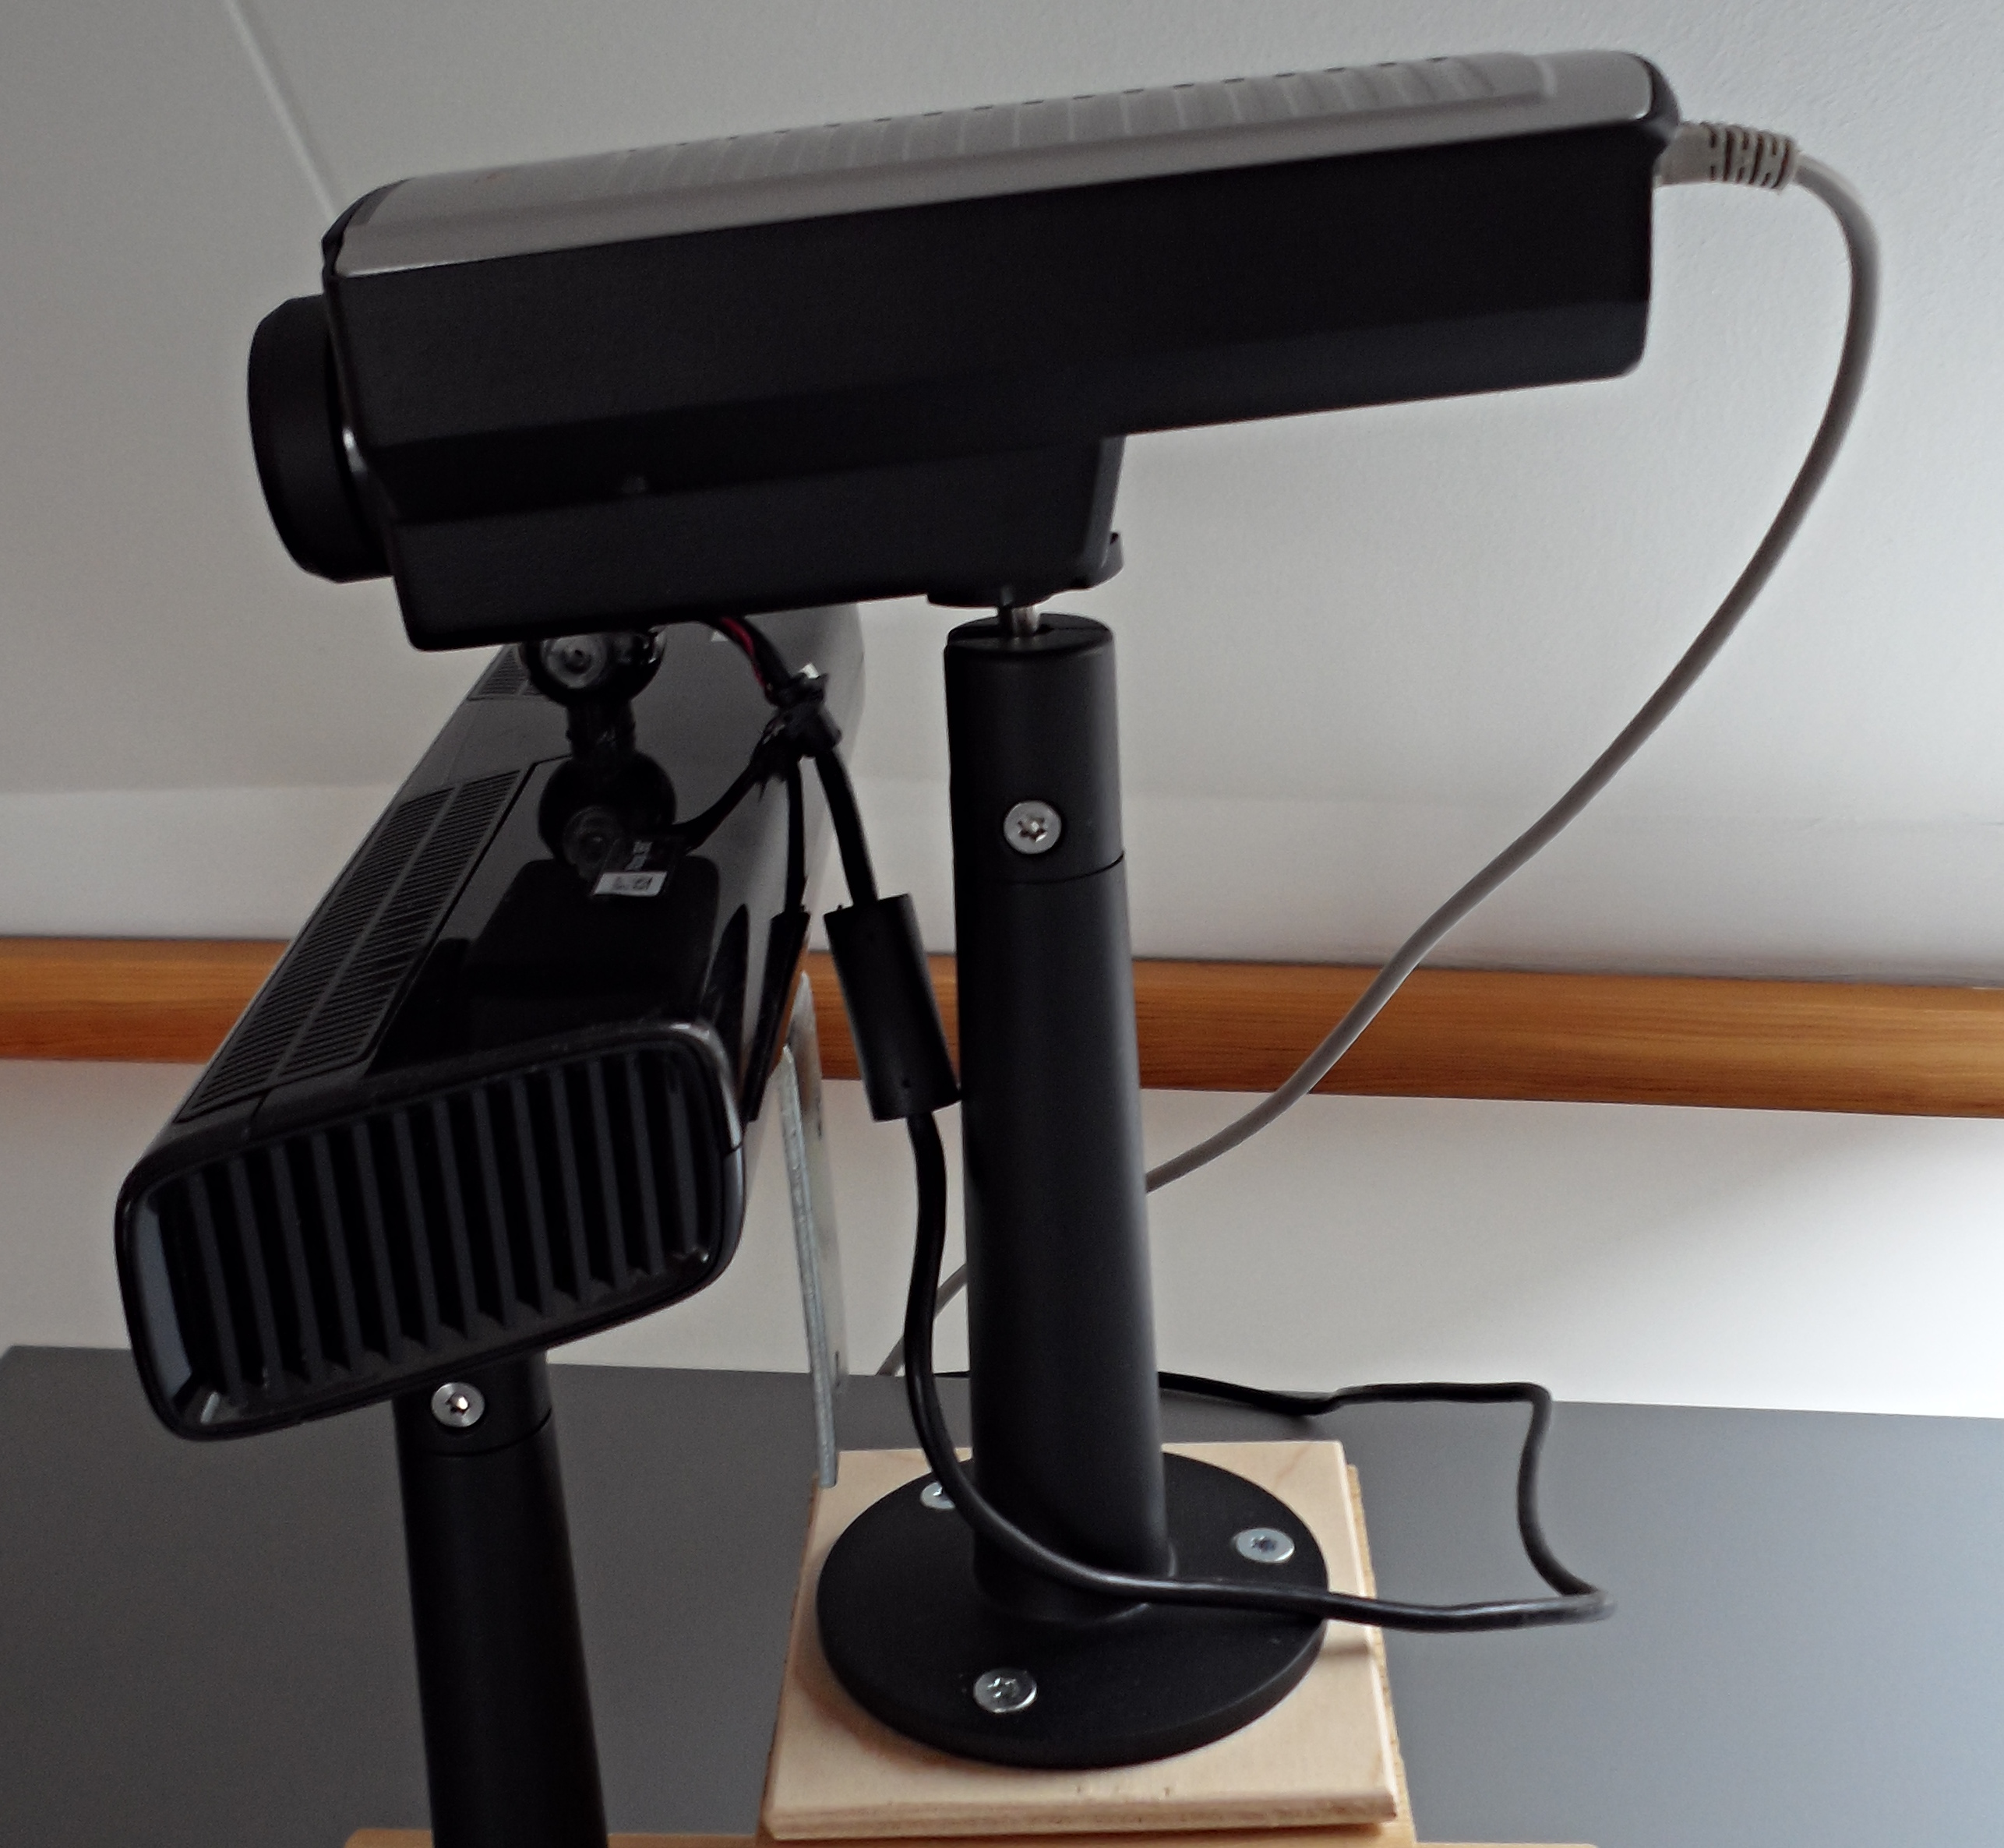
\includegraphics[width=0.25\textwidth]{pictures/camerasetup.jpg}
	\caption{Camera configuration. The RGB and thermal sensor are vertically aligned.}
	\label{fig:camerasetup}
\end{figure}

The image streams are captured using custom recording software that invokes the Kinect for Windows and AXIS Media Control SDKs. The integration of the two SDKs enables the cameras to be calibrated against the same system clock, which enables the post-capture temporal alignment of the image streams. Both cameras are able to record at 30 FPS. However, the data set is recorded at 15 FPS due to performance constraints of the recording software. 

\subsection{Multi-modal calibration}
The calibration of the thermal and RGB cameras have been accomplished using a thermal-visible calibration device inspired by \cite{vidas2012mask}. The calibration device consists of two parts; an A3-sized 10 mm polystyrene foam board is used as a backdrop and an equally sized board with cut-out squares is used as the checkerboard. Before using the calibration device, the backdrop is heated and the checkerboard plate is kept at room temperature, thus keeping a suitable thermal contrast when joined, as is seen from Figure \ref{fig:calibrationDevice}. %The depth sensor of the Kinect is factory calibrated and a subsequent calibration is thus not needed.
Using the Camera Calibration Toolbox of \cite{bouguet2004camera}, we are able to extract corresponding points in the thermal and RGB modalities. The sets of corresponding points are used to undistort both image streams and for the subsequent registration of the modalities. 

\begin{figure}[htpb]
\centering
\begin{subfigure}[b]{0.48\columnwidth}
	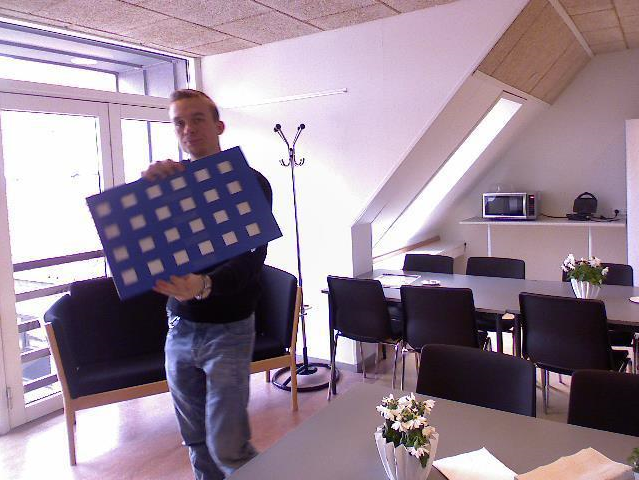
\includegraphics[width=\columnwidth]{RGB00064.png}%
	\caption{}
\end{subfigure}
\begin{subfigure}[b]{0.48\columnwidth}
	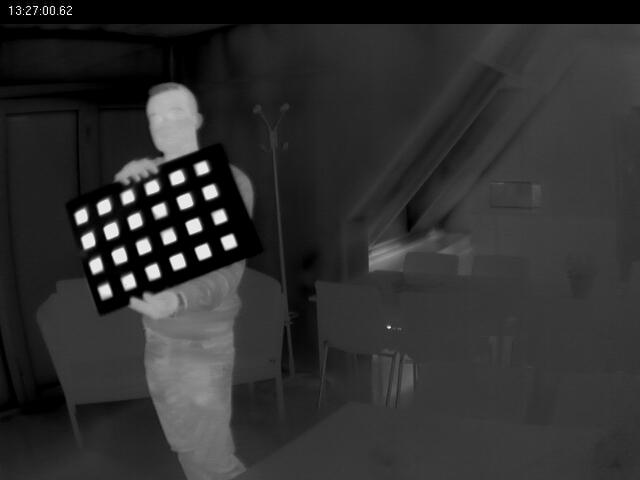
\includegraphics[width=\columnwidth]{T00064.jpg}%
	\caption{}%
\end{subfigure}
\begin{subfigure}[b]{0.48\columnwidth}
	\includegraphics[width=\columnwidth]{plane1.pdf}%
	\caption{}
\end{subfigure}
\begin{subfigure}[b]{0.48\columnwidth}
	\includegraphics[width=\columnwidth]{plane3.pdf}%
	\caption{}%
\end{subfigure}
\caption{The calibration device as seen by the (a) RGB and (b) thermal camera. The corresponding points in world coordinates is seen in (c) and the plane, which induces an homography, is overlayed in (d). Noise in the depth information accounts for the outliers in (c) and (d).}
\label{fig:calibrationDevice}
\end{figure}


\section{Registration}
\label{sec:registration}
The depth sensor of the Kinect is factory registered to the RGB camera and a point-to-point correspondence is obtained from the SDK. The registration is static and might thus be saved in two look-up-tables for $\text{RGB} \Leftrightarrow \text{depth}$. %The LUT shows to be inaccurate at positions where the Kinect cannot estimate the depth. This inaccuracy can be solved, however, by smoothing the LUT by a linear polynomial. 

The registration from $\text{RGB} \Rightarrow \text{thermal}$, $\mathbf{x} \Rightarrow \mathbf{x}'$, is handled using a weighted set of multiple homographies based on the approximate distance in space to the view that the homography represents. By using multiple homographies, we are allowed to compensate for parallax at different depths. However, the spatial dependency of the registration implies that no fixed, global registration or look-up-table is possible, thus inducing a unique mapping for each pixel at different depths.

Homographies relating RGB and thermal modalities are generated from minimum 50 views of the calibration device scattered throughout each scene. One view of the calibration device induces 96 sets of corresponding points in the RGB and thermal modality (Figure \ref{fig:calibrationDevice}c) from which a homography is computed using a RANSAC-based method. The acquired homography and the registration it establishes is only accurate for points on the plane that is spanned by the particular view of the calibration device. To register an arbitrary point of the scene, $\mathbf{x} \Rightarrow \mathbf{x}'$, the eight closest homographies are weighted according to this scheme:

\begin{enumerate}
	\item For all $J$ views of the calibration device, calculate the 3D centre of the $K$ extracted points in the image plane:
\begin{equation}
\widebar{\mathbf{X}}_{j} = \frac{\sum_{k=1}^K \mathbf{X}_{k_j}}{K} = \frac{\sum_{k=1}^K \mathbf{P}^+ \mathbf{x}_{k_j}}{K}
\end{equation}
The depth coordinate of $\mathbf{X}$ is estimated from the registered point in the depth image. $\mathbf{P}^+$ is the pseudoinverse of the projection matrix.
\item Find the distance from the reprojected point $\mathbf{X}$ to the homography centres:
\begin{equation}
\omega(j) = \lvert \mathbf{X} - \widebar{\mathbf{X}}_{j} \rvert
\end{equation}
\item Centre a 3D coordinate system around the reprojected point $\mathbf{X}$ and find $\min \omega(j)$ for each octant of the coordinate system. Set $\omega(j) = 0$ for all other weights. Normalize the weights:
\begin{equation}
\omega^*(j) = \frac{\omega(j)}{\sum_{j=1}^J \omega(j)}
\end{equation}
\item Perform the registration $\mathbf{x} \Rightarrow \mathbf{x}'$ by using a weighted sum of the homographies:
\begin{equation}
\mathbf{x}' = \sum_{j=1}^J \omega^*(j) \ \mathbf{H}_j \mathbf{x}
\end{equation}
Where $\mathbf{H}_j$ is the homography induced by the j\textsuperscript{th} view of the calibration device.
\end{enumerate}

%The spatial dependency of the registration algorithm implies that no fixed registration or look-up-table is possible. Thus, in order to register an image, one must know the spatial properties of each pixel, including depth information. 
For registering thermal points, the absence of depth information means that points are reprojected at a fixed distance, inducing parallax for points at different depths. Thus, the registration framework may be written:
\begin{align}
\text{depth} \Leftrightarrow \text{RGB} \Rightarrow \text{thermal}
\label{eq:mappingDiagram}
\end{align}

The accuracy of the registration of $\text{RGB} \Rightarrow \text{thermal}$ is mainly dependent on: 
\begin{enumerate}
	\item The distance in space to the nearest homography. %In theory, the error is proportional to the distance to the plane spanned by the homography; in practice, however, the Euclidean distance to the centre is a better estimate. 
	\item The synchronization of thermal and RGB cameras. At 15 FPS, the maximal theoretical temporal misalignment between frames is thus 34 ms. 
	\item The accuracy of the depth estimate.
\end{enumerate}
An example of the registration is seen from Figure \ref{fig:registeredImagery}. 

\begin{figure}[htpb]
\centering
\begin{subfigure}[b]{0.48\columnwidth}
	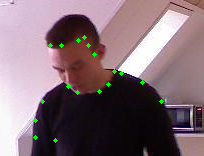
\includegraphics[width=\columnwidth]{RGBregistered.png}%
	\caption{}%
	\label{}%
\end{subfigure}
\begin{subfigure}[b]{0.48\columnwidth}
	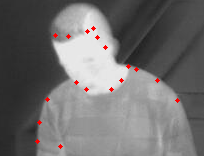
\includegraphics[width=\columnwidth]{Thermalregistered.png}%
	\caption{}%
	\label{}%
\end{subfigure}
\caption{Example of $\text{RGB (a)} \Rightarrow \text{thermal (b)}$ registration.}
\label{fig:registeredImagery}
\end{figure}

\section{Tri-modal human body segmentation}
\label{sec:trimodalhumanbodysegmentation}

Let us write $\mathbf{F}_i = \{\mathbf{C}_i, \mathbf{D}_i, \mathbf{T}_i\}$ for a determined tri-modal frame, and $\mathbf{p}$ a pixel at an arbitrary location $(x,y)$ in an image.
%continue this intro

\subsection{Extraction of masks and regions of interest} 
\label{ssec:bsbb}

The first step of our baseline is to attempt to reduce the search space. A static videocamera with fixed orientation observing an indoor scene is a common practice which enables to detect and isolate new objects entering the scene assuming that the images of the scene without new objects, known as background, exhibit some regular behavior that can be described by a statistical model. Thus, in order to perform background subtraction one has first to learn a model of the background. Once learned, this model is compared against the new incoming images and parts that do not fit are considered foreground.

\subsubsection{Background subtraction}
\label{sect:bs}
 A widely used approach for background modeling in this context is Mixture of Gaussians MOG  \cite{bouwmans2008background}, which assigns a GMM per pixel with a fixed number of components. Sometimes background presents periodically moving parts such as noise or sudden and gradual illumination changes. Such problems are often tackled with adaptive algorithms that keep learning the pixel's intensity distribution after the learning stage with a decreased learning rate. However, this also causes that intruding objects that stand still for a period of time vanish, so in our case a non-adaptive approach is more convenient.

Although this background subtraction technique performs fairly well, it has to deal with the intrinsic problems of the different image modalities. For instance, color-based algorithms may fail due to shadows, similarities in color between foreground and background, highlighted regions, and sudden lighting changes. Thermal imagery may also have this kind of problems, plus the inconvenience of temperature changes in objects. A halo effect is also observed around warm items. Regarding to depth-based approaches, they may produce misdetections due to the presence of foreground objects with similar depth to the background. However, they are more robust to lighting artifacts and shadows. Depth data is quite noisy and many pixels in the image may have no depth due to multiple reflections, transparent objects, or scattering in certain surfaces such as human tissue and hair. Furthermore, a halo effect around humans or objects is usually perceived due to parallax issues. A comparison is shown in Fig. \ref{fig:bscomparison}, where the actual foreground objects are the human and the objects on the table. As we can observe, RGB fails at extracting the human legs due to the similarities in color with the chair at the back. The thermal cue segments the human body more accurately, but includes some undesired reflections and the jar and mugs with a surrounding halo. The pipe tube is also extracted as foreground due to temperature changes along time. Despite its drawbacks, depth-based background subtraction is the one that seems to give the most accurate result. 

Therefore, the binary foreground masks of our proposed baseline are computed applying background subtraction to the depth modality previously registered to the RGB one, thus allowing us to use the same masks for both modalities.  Let us consider the depth value of a pixel at frame $i$ as $z_i$. The background model $p(z_i|BG)$ --where $BG$ represents the background -- is estimated from a training set of depth images represented by $Z$ using the $T$ first frames of a sequence such that $Z = \{z_1, \ldots, z_T\}$. This way, the estimated model is denoted by $\hat{p}(z_i| Z, BG)$, modeled as a mixture of gaussians. In particular, we use the available implementation in OpenCV of the method presented in \cite{zivkovic2004improved}, which uses an on-line clustering algorithm that constantly adapts the number of components of the mixture for each pixel during the learning stage. GMMs are further explained in section \ref{section:gmm}.

 \begin{figure}[!h]
{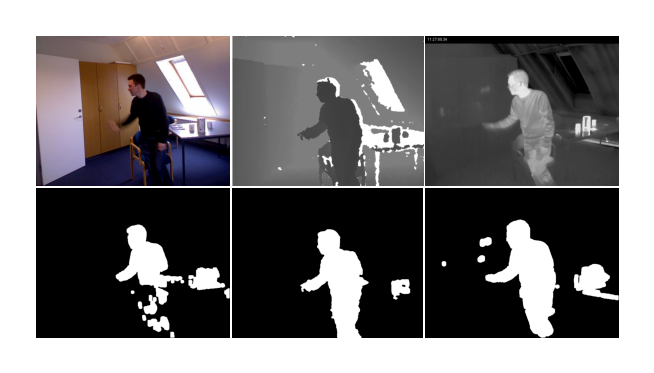
\includegraphics[width=\linewidth]{bs.eps}}
\caption{Background subtraction for different visual
modalities of the same scene (RGB, depth and thermal respectively).
\label{fig:bscomparison}}
\end{figure}

\subsubsection{Regions of interest extraction}
\label{sssec:extreg}
Once the binary foreground masks are obtained, a 2-D connected component analysis is performed using basic mathematical morphological operators and setting a minimum value for each connected component area (except in left and rightmost sides of the image which may be caused by a new incoming item) to clean the noisy output mask. 

A region of interest $r \in R$ should contain a separated person or object. However, different subjects or objects may overlap in space, resulting in a bigger component containing more than one item, for this reason each component has to be analyzed to find each item separately and therefore obtain the correct bounding boxes that surround them.

One of the advantages of the depth cue is that we can use the depth value in each range pixel to know whether an item is farther or not than other. We can assume that a given connected component belongs to just one item if its disparity distribution has a low standard deviation, that is, there is no rapid change in disparity. For those that have a greater standard deviation, Otsu's method \cite{otsu1975threshold} can be used to split the blob by automatically finding a threshold assuming a bimodal distribution. It calculates the optimal threshold separating the two classes such that their intra-class variance is minimal. We will define $\pi$ as the function that applies this method to a set of bounding boxes.

For such purpose, we define $\mathbf{c}$ as a vector containing the depth range values that correspond to a given connected component, with mean $\mu_{c}$ and standard deviation $\sigma_{c}$, and $\sigma_\mathrm{otsu}$ as a parameter that defines the maximum $\sigma_{c}$ allowed to not apply $\pi$. Note that erroneous white or black pixels do not have to be taken into account in $\mathbf{c}$ when finding the Otsu's threshold because they would change the disparity distribution, thus leading to incorrect divisions. Hence, if $\sigma_{c} > \sigma_\mathrm{otsu}$,  $\pi$ is applied. However, the assumption of bimodal distribution may not hold, so to take into account the possibility of more than two overlapping items the process is applied recursively to the divided regions in order to extract all of them. 

Once the different items are found, the regions belonging to them are labeled using a different id per item. Besides, rectangular bounding boxes are to be generated encapsulating such items individually over time, whose function is to denote the regions of interest of a given foreground mask. This way, we define the set of bounding boxes of the $i$-th frame generated from the depth-based masks as $B^\mathrm{depth}_i = \{b_{ij}\text{ }|\text{ }\forall j = \{1, \ldots, n\} \}$, being $b_{ij}$ the $j$-th bounding box and $n$ the number of bounding boxes generated in that frame, which is equal to the number of items.


\subsubsection{Correspondence to other modalities} 
\label{sssec:correspondence}
%in Section \ref{sect:bs} 
As stated previously in Section \ref{sect:bs}, depth and color cues use the same foreground masks, so we can take advantage of the same bounding boxes for both modalities. On another front, foreground masks for the thermal modality are computed using the provided registration algorithm with the depth/color foreground masks as input. For each frame, each item is registered individually to the thermal modality and then merged into one mask, preserving the same item id than depth foreground masks. This way, we achieve a one-to-one correspondence between items from both modalities and the constraint of having the same number of items in all the modalities is fulfilled. Bounding boxes are also generated the same way as done for the depth modality, which although not having the same coordinates denote the same regions of interest $R$. Henceforth, we will simply use $R$ to refer to such regions. From now on, we will use $FG = \{FG^\mathrm{color}, FG^\mathrm{depth}, FG^\mathrm{thermal}\}$ to refer to the set of foreground masks.

\subsection{Grid partitioning}
\label{ssec:gridpartitioning}

Given the precision got in the registration, particularly because of the depth-to-thermal transformation, we are not able to make a pixel-to-pixel correspondence among all the modalities. Instead, the association is made among greater information units: grid cells. 

Each region of interest $r \in R$ associated to either a segmented subject or object is partitioned in a grid of cells. We write $G_{rij}$ to refer to the position $(i,j)$ in the $r$-th region, such that $i \in \{ 1,...,n \}$ and $j \in \{ 1,...,m \}$. Regarding to the whole set of $(i,j)$-cells $\{G_{rij}\}_{\forall r \in R}$, it is denoted by $G_{ij}$.

In turn, a grid cell $G_{rij}$ consists in a set of image subregions $\{\mathbf{G}_{rij}^c\}_{\forall{c} \in \mathcal{C}}$, got from the set of imagery cues $\mathcal{C} = \{\mathrm{color}, \mathrm{depth}, \mathrm{thermal}\}$. Accordingly, $\{\mathbf{G}_{rij}^c\}_{\forall r \in R}$, the set of $(i,j)$-cells in the modality $c$, is indicated by $G_{ij}^c$.

The grid cell is the unit of information processed in the different modalities' description and classification procedures. The next section provides the details about the feature extraction computed from different visual cues at cell level.

\subsection{Feature extraction}
\label{ssec:feature extraction}

Each modality involves its own specific feature extraction/description processes. In fact, a feature extraction process can be seen as a mathematical function $f$, such that

\begin{align}
\begin{split}
f \colon & \mathbbm{R}^{n \times m} \to \mathbbm{R}^\delta \\
& \mathbf{G} \xmapsto{\phantom{\mathbbm{R}^{n \times m}}} \mathbf{d}
\end{split}
\end{align}

where $\mathbf{d}$ is a $\delta$-dimensional vector, representing the description of $\mathbf{G}$ in a certain feature space (the output space of $f$). Concretely, for the color modality two kinds of descriptions are extracted for each cell, Histogram of Oriented Gradients (HOG) and Histogram of Oriented Optical Flows (HOOF), whereas in the depth and thermal modality the Histogram of Oriented Normals (HON) and Histogram of Intensities and Oriented Gradients (HIOG) are respectively computed; hence, defining a set of four different kinds of descriptions $\mathcal{D} = \{\mathrm{HOG}, \mathrm{HOOF}, \mathrm{HON}, \mathrm{HIOG}\}$. Thus, for a particular cell $\mathbf{G}$, we come up with the set of descriptions $D_{\mathbf{G}} = \{f^d(\mathbf{G}) \;|\; \forall d \in \mathcal{D}\} = \{\mathbf{d}^d \;|\; \forall d \in \mathcal{D}\}$.

\subsubsection{Color modality}
\label{sssec:color}

The color cue is nowadays the most popular imagery modality and has been extensively used to extract a range of different feature descriptions. It is usually represented by the RGB color space, which expresses the color as a triplet $(\text{red}, \text{green}, \text{blue})$, but other models are also available. Notwithstanding its simplicity and properties, it suffer from some drawbacks such as illumination changes, shadows, camouflage, among others, which may inconvenience some tasks.

\begin{figure}
	\center
        %add desired spacing between images, e. g. ~, \quad, \qquad etc.
         %(or a blank line to force the subfigure onto a new line)
        \begin{subfigure}[b]{0.45\textwidth}
                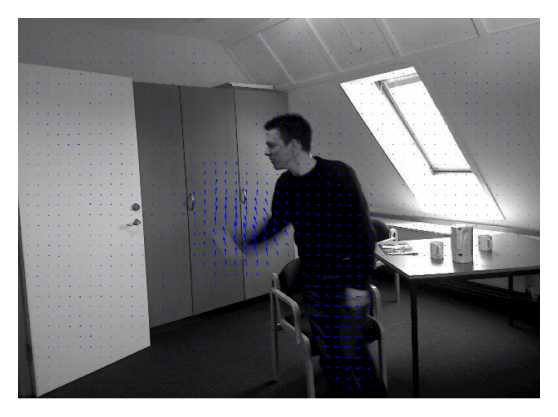
\includegraphics[width=\textwidth]{opticalflow_final.eps}
                \caption{Optical flow}
                \label{fig:opticalflow}
        \end{subfigure}
        \begin{subfigure}[b]{0.45\textwidth}
                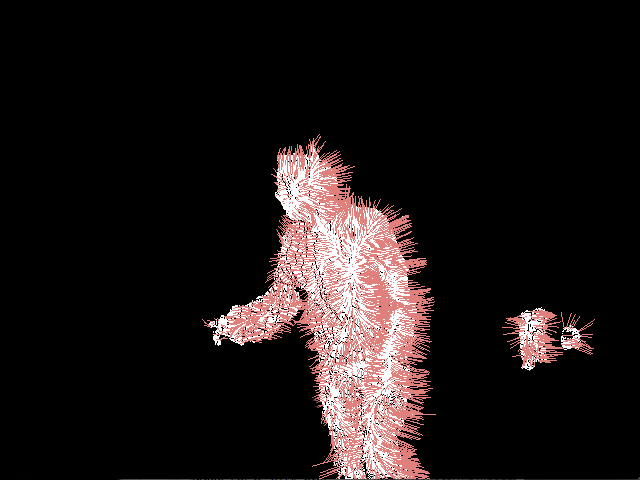
\includegraphics[width=\textwidth]{normals.png}
                \caption{Depth normals}
                \label{fig:normals}
        \end{subfigure}
        \begin{subfigure}[b]{0.45\textwidth}
                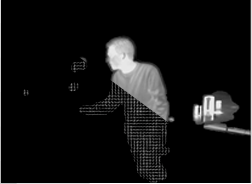
\includegraphics[width=\textwidth]{hihog.png}
                \caption{Thermal intensities and oriented gradients}
                \label{fig:thermals}
        \end{subfigure}	
        \caption{Example of descriptors computed in a frame for the different modalities: (a) represents the motion vectors using a forward scheme, that is, the optical flow orientation gives insight into where the person is moving to in the next frame; (b) the computed surface normal vectors; and (c) the thermal intensities and thermal gradients' orientations. }\label{fig:descriptors}
\end{figure}

\paragraph{Histogram of oriented gradients (HOG)}
For RGB cue, a simple implementation of HOG \cite{dalal2005histograms} is to be computed for each grid cell, known as detection window in the HOG context. Each window is resized to a $h_\mathrm{w}^\mathrm{HOG} \times v_\mathrm{w}^\mathrm{HOG}$ pixel area and divided in rectangular blocks of $h_\mathrm{b}^\mathrm{HOG} \times v_\mathrm{b}^\mathrm{HOG}$ pixels, which are in turn divided into rectangular local spatial regions called cells of size $h_\mathrm{c}^\mathrm{HOG} \times v_\mathrm{c}^\mathrm{HOG}$ pixels, thus having 4 cells per block and 8 blocks per window. We use RGB color space with no gamma correction. In order to compute the gradients, two kernels in the x and y directions with no smoothing are used for each channel so as to find and take the channel with the greatest gradient magnitude for each pixel. The gradient at point $\mathbf{p}$ of detection window is:

\begin{gather}
\mathcal{G}_\mathbf{p}^x = \mbox{[-1 0 1]} \ast \mathbf{C}_\mathbf{p} \label{eq:gx} \\[2ex]
\mathcal{G}_\mathbf{p}^y = \mbox{[-1 0 1]}^\mathrm{T} \ast \mathbf{C}_\mathbf{p} \label{eq:gy}
\end{gather}

The gradient magnitude $\mathbf{M}$ and orientation $\mathbf{\Theta}$ of the gradient at point $\mathbf{p}$ are:

\begin{gather}
\mathbf{M}_{\mathbf{p}} = \sqrt{(\mathcal{G}_{\mathbf{p}}^{\mathrm{x}})^2 + (\mathcal{G}_{\mathbf{p}}^{\mathrm{y}})^2} \label{eq:magnitude}\\[2ex]
\mathbf{\Theta}_{\mathbf{p}} = \arctan \Big(\frac{\mathcal{G}_{\mathbf{p}}^{\mathrm{y}}}{\mathcal{G}_{\mathbf{p}}^{\mathrm{x}}}\Big) \label{eq:orientation}
\end{gather}

Gradient orientation is also computed for each pixel in the dominant channel and assigned into a $\kappa$-bin histogram over each cell using unsigned gradients such that bins are evenly spaced over $0^\circ$ and $180^\circ$. As stated in \cite{dalal2005histograms}, signed contrast is uninformative for humans due to the wide range of clothing and background colors. For each gradient vector, its contribution to the histogram is given by the vector magnitude, that is, stronger magnitudes have a bigger impact on the histogram. Owing to local variations in illumination and foreground-background contrast gradient strengths vary over a wide range so cells are grouped into larger, spatially connected blocks. Hence, the information of each cell is concatenated. Then, the gradient strengths are locally normalized applying the L2-norm over each block. Block overlap is not applied in this case so as to lower the final descriptor dimensions. 

\paragraph{Histogram of oriented optical flow (HOOF)} 
Since we are working with video sequences, the color cue also allows us to obtain motion information by computing dense optical flow and describing the distribution of the resultant vectors, known as histogram of oriented optical flow \cite{dalal2006human}. The optical-flow vectors of the whole image are computed using the luminance information of the image with the Gunnar Farneb\"{a}ck's algorithm \cite{farneback2003two} available in OpenCV\footnote{\url{http://code.opencv.org.}} \cite{bradski2008learning}, which is based on modeling the neighborhoods of each pixel of two consecutive frames by quadratic polynomials. It represents the image signal in the neighborhood of each pixel by a 3-D surface and finds where the surface has moved in the next frame. As a result, a set of 2-D vectors denoting the movement of each pixel for the horizontal $\mathbf{u}$ and vertical $\mathbf{v}$ directions in the compared frames is found. It allows a wide range of parameterizations, which will be specified in Section \ref{sec:evaluation}.

 The resulting motion vectors, whose example is shown in Fig. \ref{fig:opticalflow}, are masked and quantized to produce weighted votes for local motion based on their magnitude which are locally accumulated into a $\nu$-bin histogram over each grid cell according to the signed ($0^\circ$ - $360^\circ$) vector orientations. In contrast to HOG, HOOF uses signed optical flow since the orientation provides more discriminative power. Magnitude and orientation of a motion vector at pixel $\mathbf{p}$ are calculated as in Eq. \ref{eq:magnitude} and Eq. \ref{eq:orientation} respectively.

\subsubsection{Depth modality}
\label{sssec:depth}

The grid cells in the depth modality $G^\mathrm{depth}$ are depth dense maps represented as planar images of pixels that take depth values in millimeters, thus having 3-D points in projective coordinates. From the depth representation in projective coordinates it is possible to obtain the "real world" ones by using the intrinsic parameters of the depth sensor. This conversion generates the set of 3-D point cloud structures $\mathcal{P}$ in which distances among points are actual distances -- those that can be measured in the real world. 

After having the former conversion done, for each particular point cloud $\mathcal{P}_{rij}$ (representing an arbitrary grid cell $\mathbf{G}_{rij}$) the surface normals are computed and their angles' distribution summarized in a $\delta$-bin histogram, eventually describing the cell from the depth modality point of view.

\paragraph{Histogram of oriented depth normals (HON)} 
In order to describe an arbitrary point cloud $\mathcal{P}_{rim}$ the surface normal vector for each 3-D point have to be computed first. A surface normal of a 3-D point is a perpendicular vector to a 3-D plane which is tangent to the surface in that point. Thus, the normal 3-D vector at a given point $\mathbf{p} = (p_x, p_y, p_z) \in \mathcal{P}$ can be seen as the problem of determining the normal of a 3-D plane tangent to $\mathbf{p}$. A plane is represented by the origin point $\mathbf{q}$ and the normal vector $\mathbf{n}$. From the neighboring points $\mathcal{K}$ of $\mathbf{p} \in \mathcal{P}$, we first set $\mathbf{q}$ to be the average of those points:

\begin{gather}
	\mathbf{q} \equiv \bar{\mathbf{p}} = \frac{1}{|\mathcal{K}|} \sum_{\mathbf{p} \in \mathcal{P}^{\mathcal{K}}} \mathbf{p}
\end{gather}
 
Then, the solution of $\mathbf{n}$ can be approximated using the covariance matrix $C \in \mathbb{R}^{3 \times 3}$ of the points in $\mathcal{P}_\mathbf{p}^{\mathcal{K}}$. The covariance matrix $C$ is computed as follows: 

\begin{gather}
	C = \frac{1}{|\mathcal{K}|} \sum_{i=1}^{|\mathcal{K}|} (\mathbf{p}_i - \bar{\mathbf{p}}) (\mathbf{p}_i - \bar{\mathbf{p}})^{\mathrm{T}}
\end{gather}
being $C$ a symmetric positive semi-definite matrix. Solving the next equation by means of eigenvalue decomposition:

\begin{gather}
	C \mathbf{u}_j = \lambda_j \mathbf{u}_j, \; j \in \{0,1,2\}
\end{gather}
where $\lambda_j \in \mathbb{R}$ and $\mathbf{u}_j \in \mathbb{R}^3$ represent the $j$-th eigenvalue and eigenvector of $C$ respectively, a solution for $\mathbf{n}$ is found to be the eigenvector $\mathbf{u}_j$ with the associated smaller $\lambda_j$. Formally,

% fix argmin
\begin{gather}
	\mathbf{n} = \mathbf{u}_z, \;\; \mathrm{where}\;  z = \arg\,\min_{j}{\lambda_j},\; j \in \{0,1,2\}
\end{gather}

The sign of $\mathbf{n}$ can be either positive or negative, and it can not be disambiguated from the calculations. We adopt the convention of re-orienting consistently all the computed normal vectors towards the depth sensor's viewpoint $\mathbf{z}$. Moreover, a neighborhood radius parameter $s$ will determine the cardinality of $\mathcal{K}$, that is the number of points used to compute the normal vector in each of the points in $\mathcal{P}$. The computed normal vectors over a human body region is shown in Figure~\ref{fig:normals}. Points are illustrated in white, whereas normal vectors are red lines (instead of arrows for the sake of the visual comprehension). The next step is to build the histogram describing the distribution of the normal vectors' orientations.

A 3-D normal vector got from the previous calculations is expressed in cartesian coordinates $(n_x, n_y, n_z)$. Nonetheless, a normal vector can be also expressed in spherical coordinates using three parameters: the radius, the inclination $\theta$, and the azimuth $\varphi$. In our case, the radius is a constant value, so this parameter can be omitted. Regarding $\theta$ and $\varphi$, the cartesian to spherical coordinates transformation is calculated as:

\begin{gather}	
	\theta  = \arctan{\left( \frac{n_z}{n_y} \right)},\;\;
	\varphi = \arccos{\frac{ \sqrt{(n_y^2 + n_z^2)} }{n_x}}
\end{gather}

Therefore, a 3-D normal vector can be characterized by a pair ($\theta$, $\varphi$) and the depth description of a cell consists of a pair of concatenated $\delta_\theta$-bin and $\delta_\varphi$-bin histograms, describing the two angular distributions of the body surface normals within the cell. Moreover, each of the two histograms is normalized before the concatenation, dividing by the number of elements, to end up with a relative angles frequency count.

\subsubsection{Thermal modality}
\label{sssec:thermal}

The thermal cue is a very informative feature for the task of people detection/segmentation. A pixel part of a human region gives off heat and hence a relatively large value in terms of thermal intensity.

\paragraph{Histogram of thermal intensities and oriented gradients (HIOG)} 
The descriptor got from a cell in the thermal cue $\mathbf{G}_{rij}^{\mathrm{thermal}}$ is the concatenation of two histograms. The first one is an histogram summarizing the thermal intensities, which range in the interval $[0, 255]$. The intensities are the ones in the masked region of the cell, i.e. not taking into account the background pixels. Instead, the second histogram is summarizing the orientations of thermal gradients. These gradients are computed convolving a first derivative kernel in both directions (as in Eq.~\ref{eq:gx}-\ref{eq:gy}). Then, their orientation is calculated and binned in the histogram weighted by their magnitude. Finally, the two histograms are normalized dividing by the sum of the accumulations in the bins and concatenated. We used $\upsilon_{\mathrm{i}}$ bins for the intensities part and $\upsilon_{\mathrm{g}}$ bins for the gradients' orientations.

% TODO: specify the value of \upsilon in the experiments

\subsection{Cell classification}
Since we are intended to segment human body regions, we need to distinguish those from the other foreground regions segmented by the background subtraction algorithm. These other foreground regions, apart from subjects, are the objects -- they could be other living beings, e.g. cats or dogs, though those are not considered in this work.

From the previous step, each grid cell has been described using the different descriptors $\mathcal{D}$. For the purpose of classification, we train a Gaussian Mixture Model for each grid position $(i,j)$ and kind of description $d \in \mathcal{D}$. Thus, obtaining the set of all the modeled GMMs $\mathcal{M} = \{\mathcal{M}_{ij}^{d} \;|\; \forall i \in \{1,...,n\}, \forall j \in \{1,...,m\}, \forall d \in \mathcal{D} \}$. In Fig.~\ref{fig:baseline}, the different steps of the baseline up to this point are illustrated.

% TODO: correct the baseline's figure, removing the objects' GMM

\begin{figure}[ht!]
	\centering
	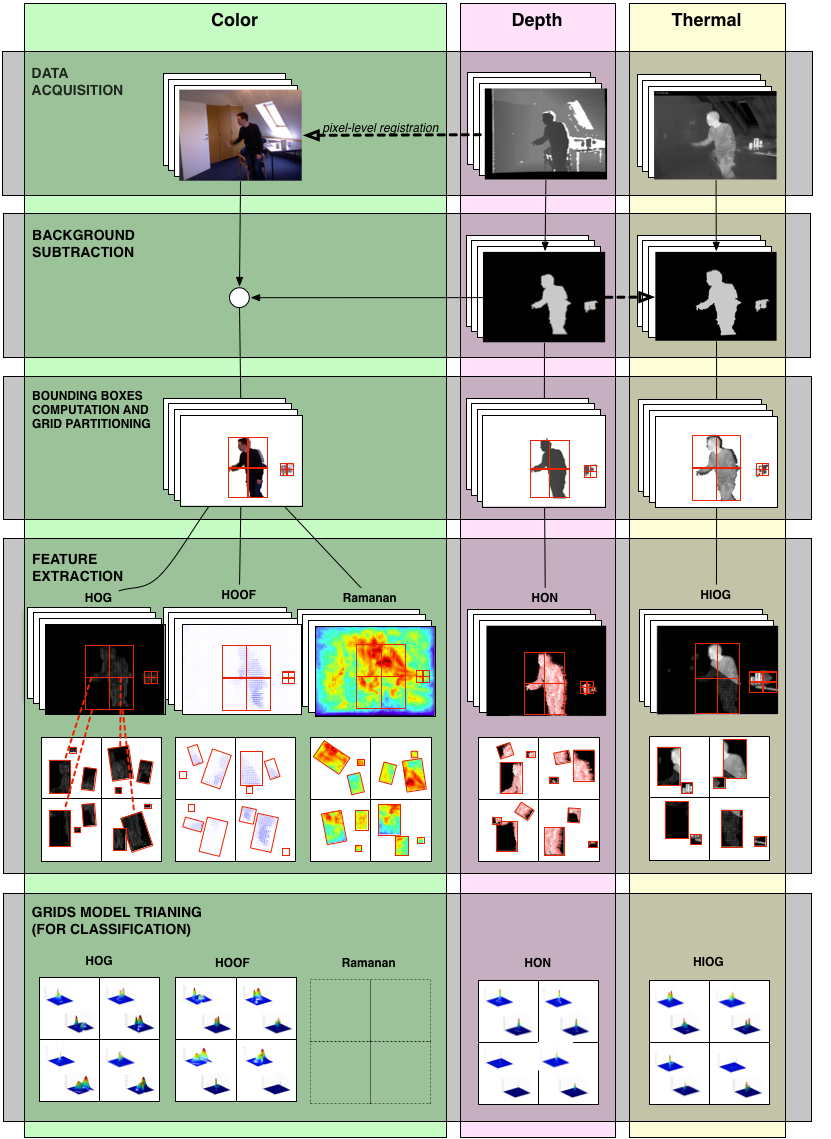
\includegraphics[width=\linewidth]{pictures/diagram.png}
	\caption{The main steps of the proposed baseline method, before reaching the fusion step.}
	\label{fig:baseline}
\end{figure}

Then, in order to predict a new unseen cell $\mathbf{G}$ to be either a subject or an object, it is evaluated the log-likelihood value in the probability density functions (PDFs) modeled for the different descriptions' mixtures. We will denote the log-likelihood values got by a particular cell $\mathbf{G}_{rij}$ in its corresponding GMMs $\{\mathcal{M}_{ij}^{d} \;|\; \forall d \in \mathcal{D}\}$ by $\{\ell_{ij}^{d} \;|\; \forall d \in \mathcal{D}\}$. The category -- either subject or object -- according $d$ is predicted by comparing the log-likelihood $\ell_{rij}^{d}$ (got by $\mathbf{G}_{rij}$ in $\mathcal{M}_{ij}^{d}$) to an experimentally selected threshold value $\tau_{ij}^d$. 

Since, for each cell, $|\mathcal{D}|$ predictions are obtained, an strategy to fuse them has to be developed. Some approaches are proposed in Section~\ref{ssec:fusion}, but first the details about the log-likelihoods computation in Gaussian Mixture Models are detailed.

\subsubsection{Gaussian Mixture Models} \label{section:gmm}

Gaussian Mixture Models (GMM) is an unsupervised learning method for fitting multiple Gaussians to a set of multi-dimensional data points\footnote{This technique uses properties of gaussians, thus its generalization to fit other functions is not straightforward.}. It is often used as a probabilistic clustering and an alternative to the k-means algorithm. As in the case of k-means, the number of components $K$ (or gaussians) in the mixture is a parameter that needs to be specified to the algorithm. The GMMs are trained using the very general Expectation-Maximization algorithm~\cite{moon1996expectation}. The goal is to end up maximizing the overall likelihood $\mathcal{L}$ of the model:

\begin{gather}
	\mathcal{L} = \prod_{\mathbf{x} \in \mathbf{X}}^{N} p(\mathbf{x})
\end{gather}
where $\mathbf{x}$ is a multi-dimensional data point (in this case representing the descriptor of an arbitrary grid cell $\mathbf{G}_{rij}^{d}$) and $p(\mathbf{x})$ is the probability of $\mathbf{x}$ being drawn from the model. This probability is the value assigned by the mixture PDF to that point, which is in fact a linear combination of $K$ gaussian PDFs:

\begin{gather}
	p(\mathbf{x}) = \prod_{k=1}^{K} p(\mathbf{x}|k) P(k)
\end{gather}
being $p(\mathbf{x}|k)$ the value assigned by the $k$-th gaussian PDF to $\mathbf{x}$ (the height of the PDF function at that point), whereas $P(k)$ is the importance, or weight, of the $k$-th component in the mixture. In fact, since the model is a mixture of gaussians, $p(\mathbf{x})$ can be expressed as the mixture of parametrized gaussian functions:

\begin{gather}
	p(\mathbf{x}) = \prod_{k=1}^{K} \mathcal{N}(\mathbf{x}|\boldsymbol{\mu}_{k}, \mathbf{\Sigma}_{k}) P(k), \\
	\mathcal{N}(\mathbf{x}|\boldsymbol{\mu},\mathbf{\Sigma}) = \frac{1}{2\pi^{\rho/2}|\mathbf{\Sigma}|^{1/2}} \exp^{-\frac{1}{2} (\mathbf{x}-\boldsymbol{\mu})^\mathrm{T} \mathbf{\Sigma}^{-1} (\mathbf{x}-\boldsymbol{\mu}) }
\end{gather}

In order to be able to predict at some point new given examples, a training procedure is needed to model the parameters of the mixture, i.e. the means $\boldsymbol{\mu} = \{ \mathbf{\boldsymbol{\mu}}_1, ..., \boldsymbol{\mu}_K \}$ and covariances matrices $\mathbf{\Sigma} = \{ \mathbf{\Sigma}_1, ..., \mathbf{\Sigma}_K \}$. This is done by the two-step procedure called Expectaction-Maximization.

\subsubsection{Expectation-Maximization: modeling a GMM}

Let be $\mathbf{X}$ the set of $\rho$-dimensional points and have initialized the parameters for the $K$ components $\boldsymbol{\mu}$ and $\mathbf{\Sigma}$ and the contribution of the components $\{P(k_1), ..., P(k_K)\}$. The first step to perform is the expectation calculation, or \emph{E-Step}, that consists on computing the $K$ posteriors for all the points $\mathbf{x} \in \mathbf{X}$. The posterior $P(k|\mathbf{x})$ is the probability the point $\mathbf{x}$ belongs to the component $k$, and it is exactly:

\begin{gather}
	p_{k\mathbf{x}} = P(k|\mathbf{x}) = \frac{\mathcal{N}(\mathbf{x}|\boldsymbol{\mu}_{k}, \mathbf{\Sigma}_{k}) P(k)}{p(\mathbf{x})}
\end{gather}

Next, it is the turn of the maximization step, or \emph{M-step}. In this step, it is supposed the assignments of individual points are known but not the model. The parameters of the components and their weights are re-estimated -- because of the previous calculations -- as:

\begin{gather}
	\hat{\boldsymbol{\mu}}_k = \frac{\sum_{\mathbf{x} \in \mathbf{X}} p_{k\mathbf{x}} \, \mathbf{x}}{\sum_{\mathbf{x} \in \mathbf{X}} p_{k\mathbf{x}}} \\
	~
	\hat{\mathbf{\Sigma}}_k = \frac{\sum_{\mathbf{x} \in \mathbf{X}} p_{k\mathbf{x}} \, (\mathbf{x}_i - \hat{\boldsymbol{\mu}}_k)(\mathbf{x} - \hat{\boldsymbol{\mu}}_k)^{\mathrm{T}} }{\sum_{\mathbf{x} \in \mathbf{X}} p_{k\mathbf{x}}}\\
	~
	\hat{P}(k) = \frac{1}{|\mathbf{X}|} \sum_{\mathbf{x} \in \mathbf{X}} p_{k\mathbf{x}}
\end{gather}

It can be proven that alternating E and M steps, the algorithm converges to at least a local maximum of overall likelihoods. A typical initialization is to start with $K$ randomly chosen data points as starting means, and equal covariance matrices. Nonetheless, convergence is sometimes slow, because of having many points laying in "plateaus". Another possibility, as it has been done in this work, is to use \emph{k-means} to have a better initialization because of a more robust estimate of the initial parameters, increasing the convergence speed and the chances of finding a better solution.

Moreover, though not explained, dealing with likelihoods may cause underflow problems in the computations. The approach to cope with this problem is to apply logarithms, that is dealing with log-likelihoods instead of likelihoods. Despite this changes some calculations re-formulated using the what is called "log-sum-exp" trick, the EM algorithm is still a valid approach to maximize the log-likelihood of the model given $\mathbf{X}$.

\subsection{Multi-modal fusion} 
\label{ssec:fusion}

Our hypothesis is that the fusion of different modalities and descriptions -- which provide a more informative and richer representation of the scenario -- will improve the final segmentation result. Such fusion can be achieved using several approaches, which are detailed below.
 
Nonetheless, before fusing the results got from the different descriptions, a normalization step is required. This normalization consists in centering and scaling the log-likelihood values corresponding to the predictions, since they are got from different descriptions' GMMs. More precisely, the log-likelihood values are centered around $\tau_{ij}^{d}$ and scaled dividing this centered value by a deviation-like term. This deviation term is simply the mean squared difference in the sample respect to $\tau_{ij}^{d}$. In such a way, the normalized log-likelihood $\varrho$ of the two categories (object and subject) conveniently differ in their sign.

\subsubsection{Description-level predictions}
\label{sssec:descriptionlevelpredictions}

Prior to the fusion step, it might be necessary to provide a prediction at grid-level (instead of cell-level) for each of the four descriptions individually, thus a strategy is needed to achieve the grid cells' predictions consensus. 

The consensus is achieved by voting, and in case of draw the magnitude of the mean normalized log-likelihoods got for both categories are compared; since normalized log-likelihood values $\varrho$ are centered at the decision threshold $\tau$, $\varrho$, which is in fact a distance to the predictor's margin, can be interpreted as a \textit{confidence} value. Thus, a grid consensus function $g(\cdot)$ is defined as follows:

\begin{gather*}\tiny
v_r^{(0)} = \sum_{i,j} \mathbbm{1}\{\varrho_{rij} < 0\} \;,\;\; v_r^{(1)} = \sum_{i,j} \mathbbm{1}\{\varrho_{rij} > 0\}  \\
\varrho_{r}^{(0)} = \sum_{(i,j) \,|\, \varrho_{rij} < 0} \varrho_{rij} \;,\;\; \varrho_{r}^{(1)} = \sum_{(i,j) \,|\, \varrho_{rij} > 0} \varrho_{rij} \\
g(r) =
\left\{
	\begin{array}{ll}
		0  & \mbox{if }  v_r^{(0)} > v_r^{(1)} \\
		\mathbbm{1}\left\{ |\varrho_{r}^{(0)}| < |\varrho_{r}^{(1)}| \right\} &  \mbox{if } v_r^{(0)} = v_r^{(1)} \\
		1 & \mbox{if }  v_r^{(0)} < v_r^{(1)} \\
	\end{array}
\right.
\end{gather*}
where $v_r^{(0)}$ and $v_r^{(1)}$ are counting the $r$ grid cells' votes for object (negative normalized log-likelihood) and subject (positive normalized log-likelihood) respectively and $\varrho_r^{(0)}$ and $\varrho_r^{(1)}$ are the accumulations of negative and positive normalized log-likelihoods respectively. Eventually, the consensus log-likelihood $\hat{\varrho}$ is also computed for further usage:

\begin{gather*}\scriptsize
\hat{\varrho}_r =
\left\{
	\begin{array}{ll}
		\frac{1}{nm / 2} \, \varrho_{r}^{(0)}  & \mbox{if }  g(r) = 0  \\
		\frac{1}{nm / 2} \, \varrho_{r}^{(1)} & \mbox{if }  g(r) = 1
	\end{array}
\right.
\end{gather*}

From this calculations, it is determined the category of a grid $r$ from each of the description's point of view and the associated consensus log-likelihoods. Having those calculated, the next step is to establish how their are fused to provide the final category of $r$.

\subsubsection{Heuristic fusion approaches}

The heuristic approaches for the fusion of the different descriptors' predictions has been analogously defined to the grid cells' consensus strategy. We defined three different approaches to tackle the fusion problem in an heuristic-like manner.

\paragraph{Grid cells' pre-consensus}

In the grid cells' pre-consensus strategy, the categories determined from the different descriptions' point of view in Section~\ref{sssec:descriptionlevelpredictions} are directly used to perform another voting and the draws are dealt using the consensus log-likelihoods. In this case, the votes are got from the different descriptions, not the cells. A fusion function $\mathcal{F}(\cdot)$ is defined as follows:

\begin{gather*}\tiny
\vartheta_r^{(0)} = \sum_{d} \mathbbm{1}\{ g^{d}(r) = 0 \} \; , \;\; \vartheta_r^{(1)} = \sum_{d} \mathbbm{1}\{ g^{d}(r) = 1 \} \\
\hat{\varrho}_r^{(0)} = \sum_{d \,|\, g^{d}(r) = 0} \hat{\varrho}_r^d \; , \;\; \hat{\varrho}_r^{(1)}  =\sum_{d \,|\, g^{d}(r) = 1} \hat{\varrho}_r^d \\
\mathcal{F}(r) =
\left\{
	\begin{array}{ll}
		0  &  \mbox{if } \vartheta_r^{(0)} < \vartheta_r^{(1)}   \\
		\mathbbm{1}\left\{ | \hat{\varrho}_r^{(0)} | < | \hat{\varrho}_r^{(1)} | \right\} &  \mbox{if } \vartheta_r^{(0)} = \vartheta_r^{(1)}   \\
		1 &  \mbox{if } \vartheta_r^{(0)} > \vartheta_r^{(1)}   \\
	\end{array}
\right.
\end{gather*}
where $\vartheta_r^{(0)}$ and $\vartheta_r^{(1)}$ are counting the descriptions' votes for object ( category in the cells' consensus function $g(\cdot)$ and subject (1 category in the cells' consensus function $g(\cdot)$) and $\hat{\varrho}_r^{(0)}$ respectively and $\hat{\varrho}_r^{(1)}$ are the accumulations of negative and positive consensus log-likelihoods respectively.

\paragraph{Grid cells' post-consensus}

An alternative approach to the pre-consensus is simply performing the fusion at cell-level by voting first and, then, performing another voting to achieve the cells' consensus.

%\begin{gather*}\tiny
%\vartheta_{rij}^{(0)} = \sum_{d} \mathbbm{1}\{ \ell_{rij}^d < 0 \} \; , \;\; \vartheta_{rij}^{(1)} = \sum_{d} \mathbbm{1}\{ \ell_{rij}^d > 0 \} \\
%\ell_{rij}^{(0)} = \sum_{d \,|\, \ell_{rij}^d < 0} \ell_{rij}^d \;,\;\; \ell_{rij}^{(1)} = \sum_{d \,|\, \ell_{rij}^d > 0} \ell_{rij}^d \\
%h(r,i,j) =
%\left\{
%	\begin{array}{ll}
%		0  & \mbox{if }  \vartheta_{rij}^{(0)} > \vartheta_{rij}^{(1)} \\
%		\mathbbm{1}\left\{ |\ell_{rij}^{(0)}| < |\ell_{rij}^{(1)}| \right\} &  \mbox{if }  \vartheta_{rij}^{(0)} = \vartheta_{rij}^{(1)} \\
%		1 & \mbox{if }  \vartheta_{rij}^{(0)} < \vartheta_{rij}^{(1)} \\
%	\end{array}
%\right.\\
%\hat{\ell}_{rij} =
%\left\{
%	\begin{array}{ll}
%		\frac{1}{|\mathcal{D}| / 2} \, \ell_{rij}^{(0)}  & \mbox{if }  g(r) = 0  \\
%		\frac{1}{|\mathcal{D}| / 2} \, \ell_{rij}^{(1)} & \mbox{if }  g(r) = 1
%	\end{array}
%\right.\\
%v_r^{(0)} = \sum_{i,j} \mathbbm{1}\{h(r,i,j) = 0\} \;,\;\; v_r^{(1)} = \sum_{i,j} \mathbbm{1}\{h(r,i,j) = 1\}  \\
%\ell_{r}^{(0)} = \sum_{(i,j) \,|\, h(r,i,j) = 0} \ell_{rij}^{(0)} \;,\;\; \ell_{r}^{(1)} = \sum_{(i,j) \,|\, h(r,i,j) = 1} \ell_{rij}^{(1)} \\
%\mathcal{G}(r) =
%\left\{
%	\begin{array}{ll}
%		0  &  \mbox{if } \vartheta_r^{(0)} < \vartheta_r^{(1)}   \\
%		\mathbbm{1}\left\{ | \hat{\ell}_r^{(0)} | < | \hat{\ell}_r^{(1)} | \right\} &  \mbox{if } \vartheta_r^{(0)} = \vartheta_r^{(1)}   \\
%		1 &  \mbox{if } \vartheta_r^{(0)} > \vartheta_r^{(1)}   \\
%	\end{array}
%\right.
%\end{gather*}


\paragraph{Distance-based fusion and cells' post-consensus}

The difference between this last approach and the former one is the way to fuse the information at description-level. While the former was determining the category at cell-level by voting, thus not taking into account the normalized log-likelihood value but the sign (except for draw cases), this later approach seeks to base in the magnitude of the normalized log-likelihood value's in the descriptions' fusion process. As in \textit{cells' post-consensus} the grid cells' decisions are consensued by voting.

The problem with the heuristic fusion approaches is the impossibility determining the importance of each of the description-level predictions when fusing or the relevance of the cell predictions when performing the grid cells' consensus. For instance, the thermal cue could be providing the most reliable description or the grid cells comprising the upper body could provide more reliable results than the lower body ones. In this sense it is proposed the next approach, which consists in using state-of-the-art statistical learning algorithms to get grid category predictions somehow from the GMMs' predictions, and hopefully achieve a better performance in terms of subject detection than the previous described approaches.

\subsubsection{The learning-based fusion approach}

As before, the category of a grid $r$ is intended to be predicted, but instead of directly making use of the descriptors computed from the different modalities, the predictions got from the GMMs in different cells and each kind of description are taken advantage of. This approach follows the Stacked Learning scheme \cite{cohen2005stacked, gatta2011multi}, which involves training a new learning algorithm combining previous predictions obtained with other learning algorithms. More precisely, each grid $r$ is represented by a vector $\mathbf{v}_r$ of normalized log-likelihoods:

$$\mathbf{v}_r = (\varrho_{r11}^{(1)}, ..., \varrho_{rNM}^{(1)}, ..., \varrho_{r11}^{(|\mathcal{D}|)}, ..., \varrho_{rNM}^{(|\mathcal{D}|)}, y_r)$$
where $y_r$ is the actual category of the $r$ grid. Using this vectorized-form representation, the data sample containing the $R$ instances is built. Therefore any supervised learning algorithm can be used to try to learn from these data and infer more reliable predictions than using the previous handcrafted heuristics. 

Among many existing state-of-the-art supervised learning algorithms for classification, we selected three of them: Adaptive Boosting (gentle version)~\cite{freund1999short}, Artificial Neural Networks (Multi-Layer Perceptron~\cite{rosenblatt1961principles} with both sigmoidal and radial basis activation function), and Support Vector Machines~\cite{cortes1995support} (linear and radial basis function kernels).

%\paragraph{Adaptive Boosting (AdaBoost)} is a learning meta-algorithm that builds a strong classifiers by combining many weak classifiers. This combination can be a simple weighted sum of the weak classifiers' outputs. The idea is the aggregation weak predictions (barely better than random guessing) boosts the strong decision. Decision trees are the most popular weak classifiers used in boosting schemes, ...
%
%\paragraph{Multi-Layer Perceptron (MLP)} is a feed-forward artificial neural network model, graph-like represented, which maps a multi-dimensional input to the proper multi-dimensional output~\cite{rosenblatt1961perceptrons}. A MLP consists of more than two fully connected layers of nodes (or neurons). Particularly, the MLP aggregates and stacks many perceptrons in order to, respectively, deal with the output multi-dimensionality and the non-linear separability of the data. Each layer is composed of neurons (except for the input layer), each of them fully connected to the next one; that is, a given neuron receives the input of all the neurons of the previous layer's neurons and in turn this neuron emits a synchronous signal directed to each of the neurons in the next layer. The training of an artificial neural network model consists in setting the weights in the neural connections so as to maximize the prediction performance, and it is typically done with the so-called backpropagation algorithm~\cite{rumelhart1986learning}; this technique iteratively inputs data to the network and backpropagates the error got in the output, adapting somehow the weights so as to minimize the error the output error is minimized after each iteration.
%
%While the number of neurons in the hidden layer $h$ is a parameter that has to be selected, the number of neurons in both the input layer and output layer are determined, respectively, by the input data dimensionality and the number of output variables that need to be predicted (number of classes in classification problems). Other model parameters are the number of epochs $e$ (iterations of error backpropagation), and the weight update factor $\alpha$.
%
%% TODO: add to the bib: rosenblatt1961perceptrons, rumelhart1986learning
%
%\paragraph{Support Vector Machine (SVM)} is a non-probabilistic supervised binary classifier that learns a model which represents the instances as points in space, mapped in such a way that instances of different classes are separated by a hyperplane in a high dimensional space. However, if the dataset is not linearly separable in that space the hyperplane will fail in classifying properly. This can be solved by mapping the dataset instances into a higher dimensional space using a kernel function, thus making easier the dataset division \cite{hearst1998support}. 
%
%In particular, our baseline includes linear kernel and radial basis function (RBF)\footnote{The SVM models has been trained using the available implementation of the LibSVM\footnote{\url{http://www.csie.ntu.edu.tw/~cjlin/libsvm/ }} library \cite{chang2011libsvm}.}. Linear SVM just requires one parameter, the penalty parameter $\zeta$, which specifies a trade-off between model complexity and misclassification of training examples and can take values in the interval $[0, inf)$. Higher values of $\zeta$ causes closer fitting to the training set, which may tend to overfitting. The performance of the RBF kernel is also influenced by the $\gamma$ parameter, which controls the shape of the separating hyperplane. Higher values usually increase the number of support vectors. Weights $\mathbf{w}$ obtained from linear SVM represent the hyperplane used to separate between classes, but they can also give us an insight of the level of importance or level of influence that each feature has when classifying the instance \cite{guyon2003introduction}.

%Such parameters have influence on the model accuracy, for that reason a proper parameter selection has to be performed


\section{Evaluation}
\label{sec:evaluation}
The proposed method is evaluated on a data set with a total of 11537 frames, of which 5724 frames are annotated as this requires a significant amount of resources. Sample imagery of the scenes is pictured in Figure \ref{fig:samplescenes} whereas Table \ref{tab:scenes} shows the number of annotated frames and the depth range. Activity in scene 1 and 3 is using the full depth range of the Kinect sensor whereas activity in scene 2 is constrained to a depth range of $\pm 0.250$ m. Scene 1 and 2 are situated in a closed meeting room with little natural light to disturb the depth sensing, whereas scene 3 is situated in a area with wide windows and a substantial amount of sunlight.

\begin{figure}[htbp]
	\centering
		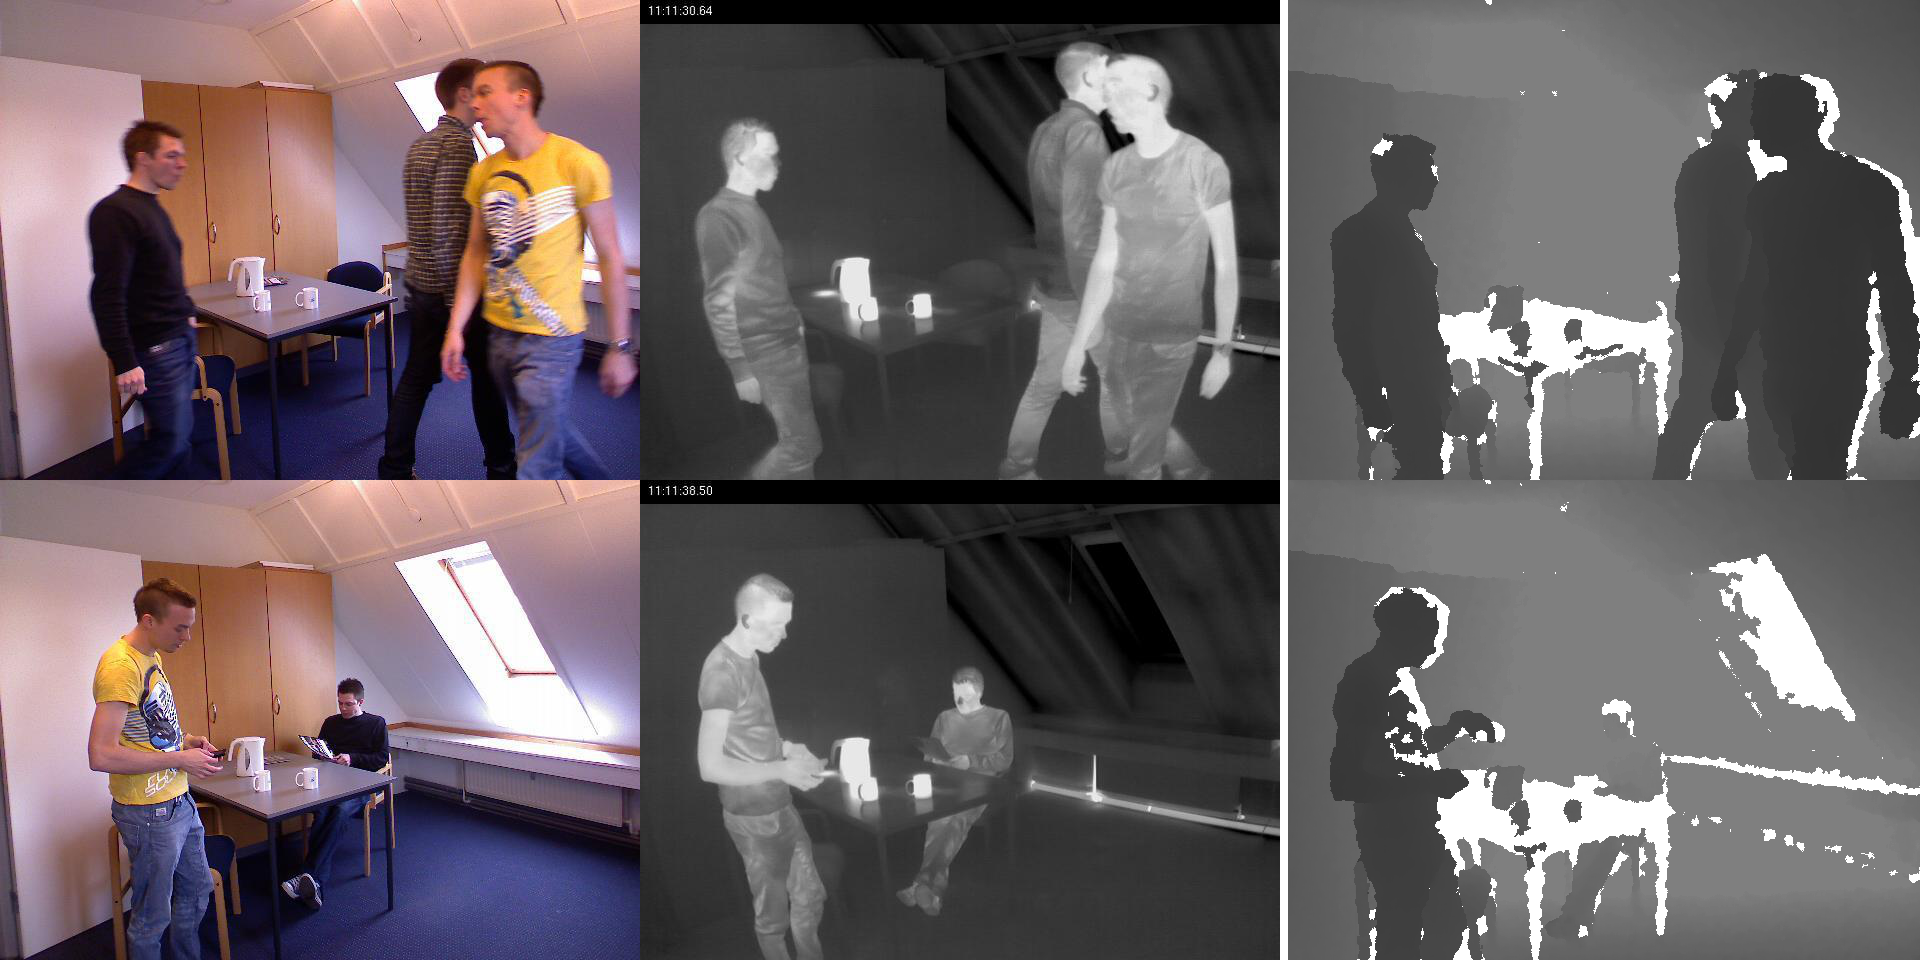
\includegraphics[width=0.48\textwidth]{Selection/1.png}
		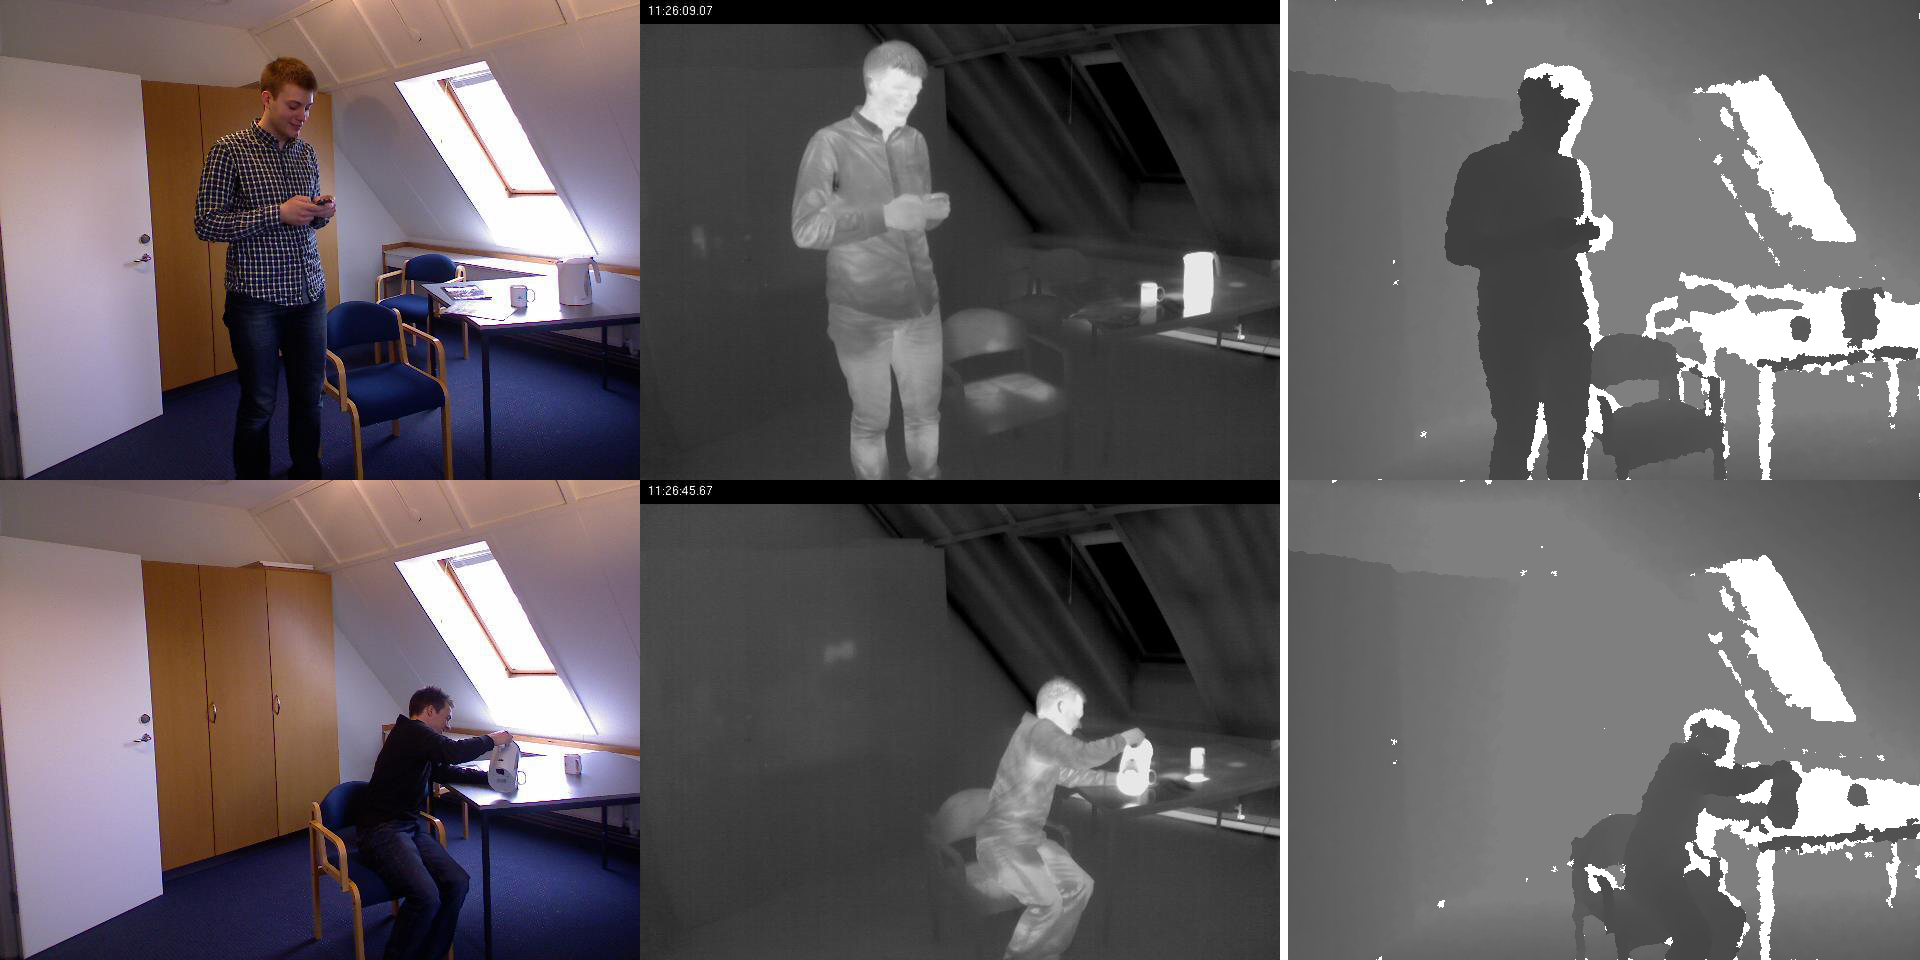
\includegraphics[width=0.48\textwidth]{Selection/2.png}
		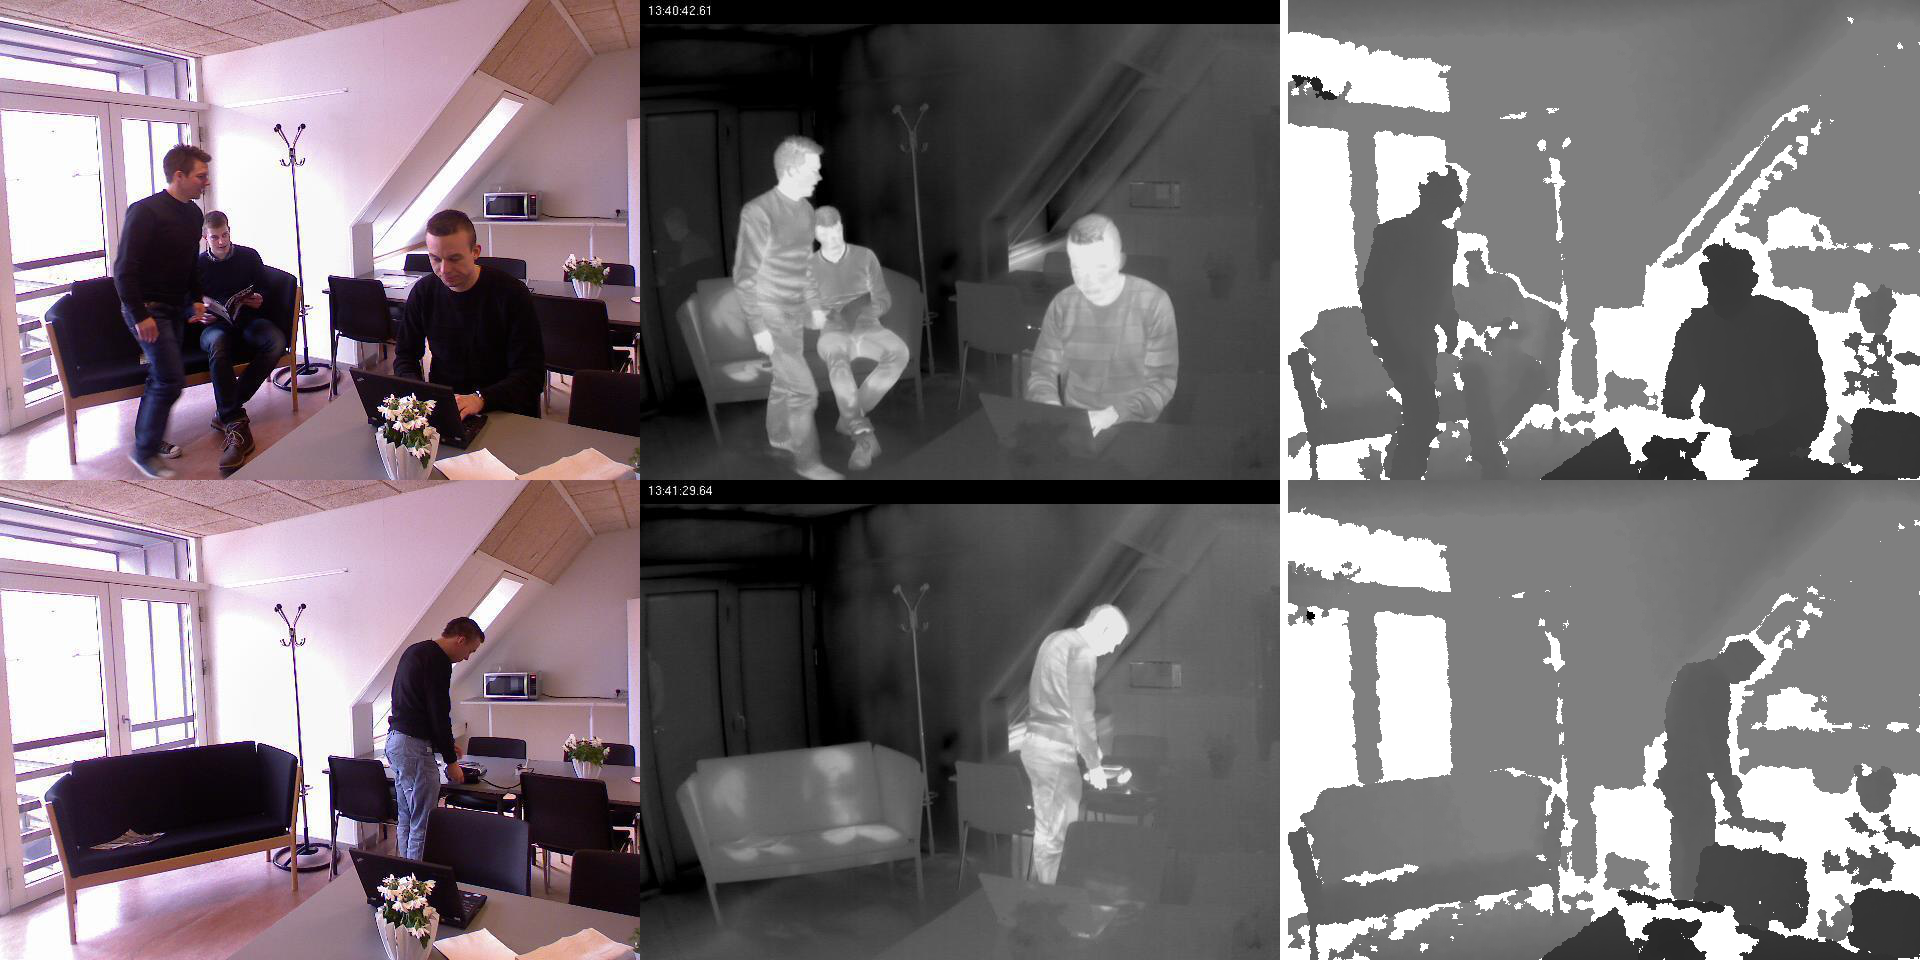
\includegraphics[width=0.48\textwidth]{Selection/3.png}
	\caption{Two views of each of the three scenes shown in the RGB, thermal, and depth modalities, respectively.}
	\label{fig:samplescenes}
\end{figure}

\begin{table}[htpb]
\centering
\begin{tabular}{llll}
\hline
Scene & Frames 	& Annotated frames 	& Depth range \\ \hline
1 		& 4693		& 1767	 						& 1-4 m \\
2 		& 2216		& 2016	 						& 1.4-1.9 m \\
3 		& 4628		& 1941	 						& 1-4 m \\ 
\hline
\end{tabular}
\caption{Annotated number of frames and spatial constraints of the scenes.}
\label{tab:scenes}
\end{table}

\subsection{Annotation}
%The frames are annotated using a pixel annotator tool ***ANDREAS TEXT HERE****
%
 %For each scene, human objects are annotated in the RGB modality. Each person is given a unique ID which he maintains throughout the scene. To obtain the corresponding masks in the thermal and depth modalities, the RGB masks are mapped using the registration algorithm of Section \ref{sec:registration}.
The acquired video was manually annotated frame-by-frame in a custom annotation program called Pixel Annotator. The dataset contains a large number of frames divided over a number of different sequences. All sequences have three modalities: RGB, depth, and thermal. The focus of the annotation has been on the people in the scene and a mask-based annotation philosophy has been employed. That means that each person is covered by a mask and each mask (person) has a unique ID, which is consistent over frames. In this way the dataset can be used not only for background subtraction, but also for tracking and re-identification purposes. Since the main purpose of the dataset is background subtraction, a pixel-level annotation scheme was necessary - bounding boxes would not be sufficient.
 
As seen from Figure \ref{fig:pixelannotator}, Pixel Annotator provides a view of each modality with the current mask overlaid, as well as a raw view of the mask. It implements the registration algorithm described above so that the annotator can judge whether the mask fits in all modalities. Because the modalities are registered to each other, there is not specific masks for each modality, but a single mask for all.

\begin{figure}%
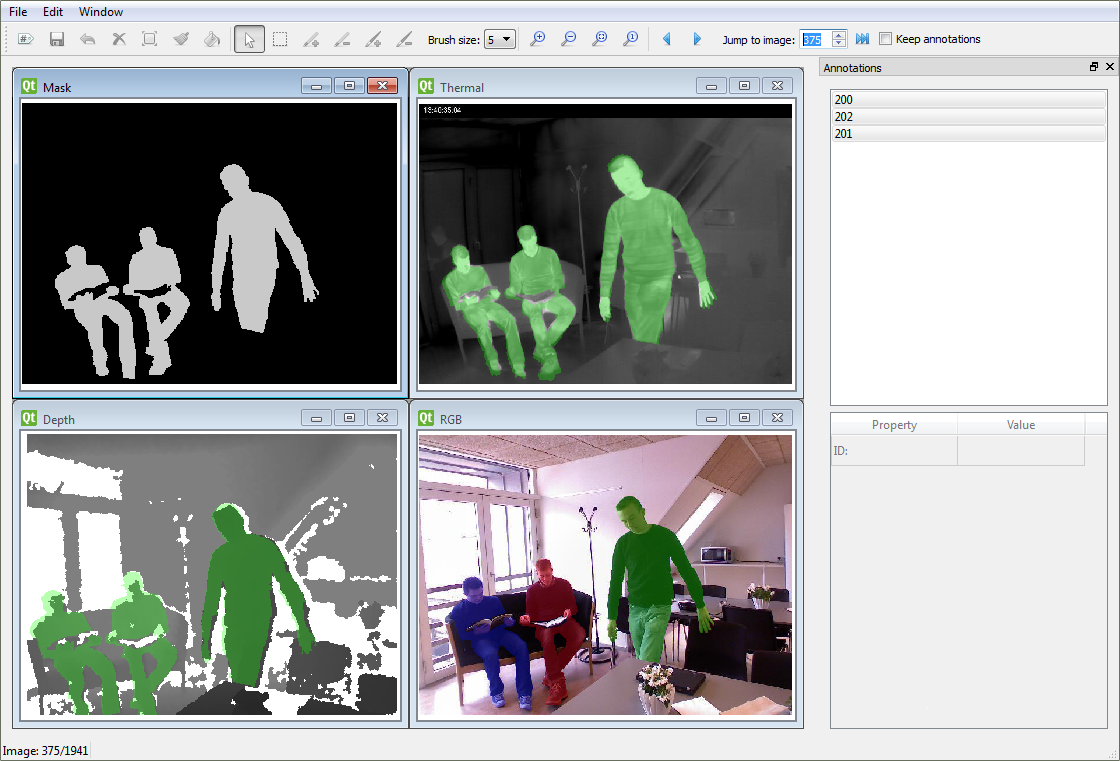
\includegraphics[width=0.48\textwidth]{pixelannotator2.png}%
\caption{Pixel Annotator showing the RGB masks and the corresponding, registered masks in the other views.}%
\label{fig:pixelannotator}%
\end{figure}

Each annotation can be initialized with an automatic segmentation using the GrabCut algorithm \cite{rother2004grabcut} to get quickly off the ground. Then Pixel Annotator provides pixel-wise editing functions to further refine the mask. Each annotation is associated with a numerical ID, and can have an arbitrary number of property fields associated with it. They can be boolean or contain strings, so advanced annotation can take place, all the way from simple occluded/not occluded fields to fields describing the current activity. Pixel Annotator is written in C++ on the Qt framework and is fully cross-platform compatible.

The data set and the registration algorithm is freely available at \cite{vapgroup}.

\subsection{Parameters and settings}
\label{ssec:parametersandsettings}

After some experiments regarding the use of Otsu's threshold in the background subtraction and generation of bounding boxes stage, we set $\sigma_\text{otsu} = 8.3$ for a connected component area of at least 0.1\% of the image, or  $\sigma_\text{otsu} = 12$ for other cases. % Ref or convincing rational explanation?

Since it is not possible to have a pixel-to-pixel correspondence among modalities, we define the correspondence at a grid cell level. The grids have been partitioned in $m \times n$ cells, being $m = 2$ and $n = 2$. The main idea of the grid partitioning is to reduce the variability of the regions in each GMM. At the same time, they are large enough to not condition the eventually computed overlap measure.

For the HOG descriptor, we defined $H_\text{w} = 64 \times 128$, $H_\text{b} = 32 \times 32$, $H_\text{c}=16 \times 16$, and $H_{h} = 9$. The information of each cell is concatenated resulting in a vector of 36 values per block. This brings the final vector size of a grid cell to 4 blocks vertically $\times$ 2 blocks horizontally $\times$ 4 cells per block $\times$ 9 bins per cell, making a total of 288 components/dimensions. % Ref or convincing rational explanation?

In order to compute the optical flow, and based on the tests performed in \cite{brkic2013combining}, we set the parameters of the given implementation according to the values that gave the best performance. In particular, the averaging window size was set to 2, the size of the pixel neighborhood considered when finding polynomial expansion in each pixel was set to 5 and the standard deviation of the Gaussian that is used to smooth derivatives used as a basis for the polynomial expansion to 1.1.  The remaining parameters were set to their default OpenCV values. For the motion descriptor (HOOF), we defined $V_\text{b}$ = 8, to finally produce an 8-dimensional feature vector. 

Then, for the depth descriptors (HON), we defined $\theta_{I} = 8$ and $\phi_{G} = 8$, whereas for the thermal descriptors (HIOG), we defined $T_{I} = 8$ and $T_{G} = 8$. A very large number of bins is not convenient for generalization. Besides, we wanted the number of bins describing orientations in the different descriptions to coincide for comparison purposes in the later experiments; and 8 bins for describing normal vectors' orientations seem a quite reasonable amount of bins in view of the depth sensor's noisy measurements. In fact, to deal with this noise the neighborhood radius $s$ in the normal computation needs to be adjusted. Thus, we empirically selected between two values ($\{0.02, 0.04\}$) the one performing better (according to our validation measures next explained), that in this case has been $s = 0.02$. That demonstrated that larger values would be providing worse performances, while smaller ones are not reasonable because affects the orientations.

Other more sensitive parameters, specially the ones related to learning algorithms, have been experimentally selected. In the GMM-related experiments, $k = \{2,3, ..., 9, 11, 13\}$ and $\tau = (-2,2)$ (in 32 equal width steps). In the AdaBoost experiment, the number of possible weak classifiers and the weight trimming rates  $\{10, 20, 50, 100, 200, 500, 1000\}$ and $\{0, 0.7, 0.75, 0.8, \ldots, 1\}$ respectively; in the MLP, $h = \{2, 5, 10, \ldots, 50, 60, \ldots, 100\}$; and, in the SVM, $\zeta = \{1e-7, 1e-6, \ldots, 1e4\}$ and $\gamma = \{1e-7, 1e-6, \ldots, 1e2\}$.


\subsection{Experimental methodology and validation measures}
\label{ssec:validation}

The proposed baseline has been validated by means of cross-validation (CV). For this purpose, we divided the dataset at frame-level in 10 non-overlapping partitions, with each partition containing perhaps a slightly different number of frames but the same number of subject regions. This ensures a fair training of the models across different folds, i.e. training the models with the same number of subject examples. In order to do that, we simply stratified the partitions by the number of appearing subject regions in the associated groundtruth masks. The dataset could not be directly partitioned at region-level, because a per-frame overlap measures the performance of our method.

In addition, we performed a model selection in each training partition to find the optimal values for the GMMs' experimental parameters ($k$ and $\tau$). We used again the cross-validation strategy, but with a smaller number of partitions (3). In each inner fold, a grid search has been carried out to measure the performance of each $k$-$\tau$ combination. The optimal combination, i.e. the one performing better in average across these inner folds, was used to train the final models eventually validated in the test partitions. In this case, and since we measured the subject prediction accuracy, the data was partitioned at region-level.

The parameters of the learning-based fusion's classifiers were also selected in each iteration of outer CV, and this is done in the exact same inner 3-fold cross-validation partitions. While the selection of $k$ and $\tau$ were  enough exhaustive, the parameters involved in these supervised learning algorithms often require an even more exhaustive search to fine tune their values. A common strategy to keep the number of parameter combinations manageable is to perform a two-level grid search, which consists of a first coarse grid search followed by a second narrow grid search around the coarse's optimal values.

% A table of results here

As said before, we have used an overlap measure in order to compare the similarity between the groundtruth masks and the predicted masks, thus assessing the performance of the proposed baseline. Concretely, the Jaccard Index \cite{tan2002selecting}, also known as the Jaccard similarity coefficient. The degree of overlap between two binary sets $A$ and $B$ is computed as the ratio between the size of the intersection divided by the size of the union:
\begin{equation} \label{eq:jaccard}
overlap(A, B) = \frac{|A \cap B|}{|A \cup B|}
\end{equation}

This measure takes values in $[0,1]$, 0 meaning no overlap and 1 meaning perfect agreement between sets. $GT$ represents connected components of the ground truth binary masks, and $\hat{S}$ those of predicted binary masks from the different modalities individually or from the different fusion approaches. For each frame, the overlap is computed per person id and connected component, in such a way that connected components that have the same person id  or are connected in the ground truth constitute a set $A$, and they are compared to the blobs that coincide in the predicted binary masks, which constitute a set $B$. The overlap of each frame is then averaged by the number of sets found. It is therefore a pessimistic measure because a very tiny blob misclassified as a person in the predicted binary masks will account for 0 overlap, thus decreasing the mean overlap of the frame, so it can be considered as a lower bound on how accurate the prediction is. The final overlap is computed as the mean overlap of all frames having at least one blob, whether they be in the ground truth or in the predicted binary mask.

As commented in Section~\ref{sect:bs}, the depth cue suffers from a halo effect around people or objects, thus complicating an accurate pixel-level segmentation at blob contours when applying background subtraction. This lack of accuracy is also caused by possible distortions, noise or other problems, and decreases the final overlap. Hence, a \emph{do not care region} (DCR) is often used. Such region is taken per frame by centering a morphology operator of different sizes at the ground truth binary masks blob contours and subtract it from those masks and from the predicted ones to compute the overlap. This way, we can compare the effect of using a growing DCR to the actual overlap.

\section{Experimental results}
\label{ssec:experimentalresults}

As explained in the last section, we assess the performance of the proposed baseline using both a detection accuracy and the Jaccard overlap measure (Eq. \ref{eq:jaccard}). Figure \ref{fig:overlapgraph} depicts the obtained overlap for individual predictions and fusion predictions with different fusion approaches. Tables \ref{table:individual} and \ref{table:linearstacked} are included to compare the differences between using the descriptors separately and after fusing them. Notice that in plots showing fusion results, only two cases are considered, owing to color and depth modalities share the same original $FG$ masks.

\begin{table}[h]\footnotesize
\center
\caption{Overlap results of the individual predictions for each description}
\label{table:individual}
\begin{tabular}{|l|l|l|l|l|l|}
\hline
&\textbf{HOG}&\textbf{SM}&\textbf{HOOF}&\textbf{HIOG}&\textbf{HON}\\\hline
\textbf{0}&62.10 \% &63.12 \%&56.97 \%&46.35 \%&56.76 \%\\\hline
\textbf{1}&64.71 \%&65.85 \%&59.41 \%&47.99 \%&59.09 \%\\\hline
\textbf{3}&67.59 \%&69.02 \%&62.13 \%&50.85 \%&61.70 \%\\\hline
\textbf{5}&68.65 \%&70.40 \%&63.20 \%&53.02 \%&62.77 \%\\\hline
\textbf{7}&68.65 \%&70.72 \%&63.28 \%&54.45 \%&62.94 \%\\\hline
\end{tabular}
\end{table}


\begin{table}[h]\footnotesize
\center
\caption{Overlap results of fusion using Stacked Linear SVM for each modality}
\label{table:linearstacked}
\begin{tabular}{|c|c|c|}
\hline
\textbf{DCR}&\textbf{Thermal}&\textbf{Color/Depth}\\\hline
\textbf{0}&49.64 \%&64.65 \%\\\hline
\textbf{1}&51.33 \%&67.39 \%\\\hline
\textbf{3}&54.29 \%&70.43 \%\\\hline
\textbf{5}&56.56 \%&71.58 \%\\\hline
\textbf{7}&58.11 \%&71.63 \%\\\hline
\end{tabular}
\end{table}

%Linear SVM is used as baseline classifier. It offers good performance relative to other linear classifiers and %fast to run.


 \begin{figure}[H]
	 \centering
	 \begin{subfigure}[b]{0.47\textwidth}
 		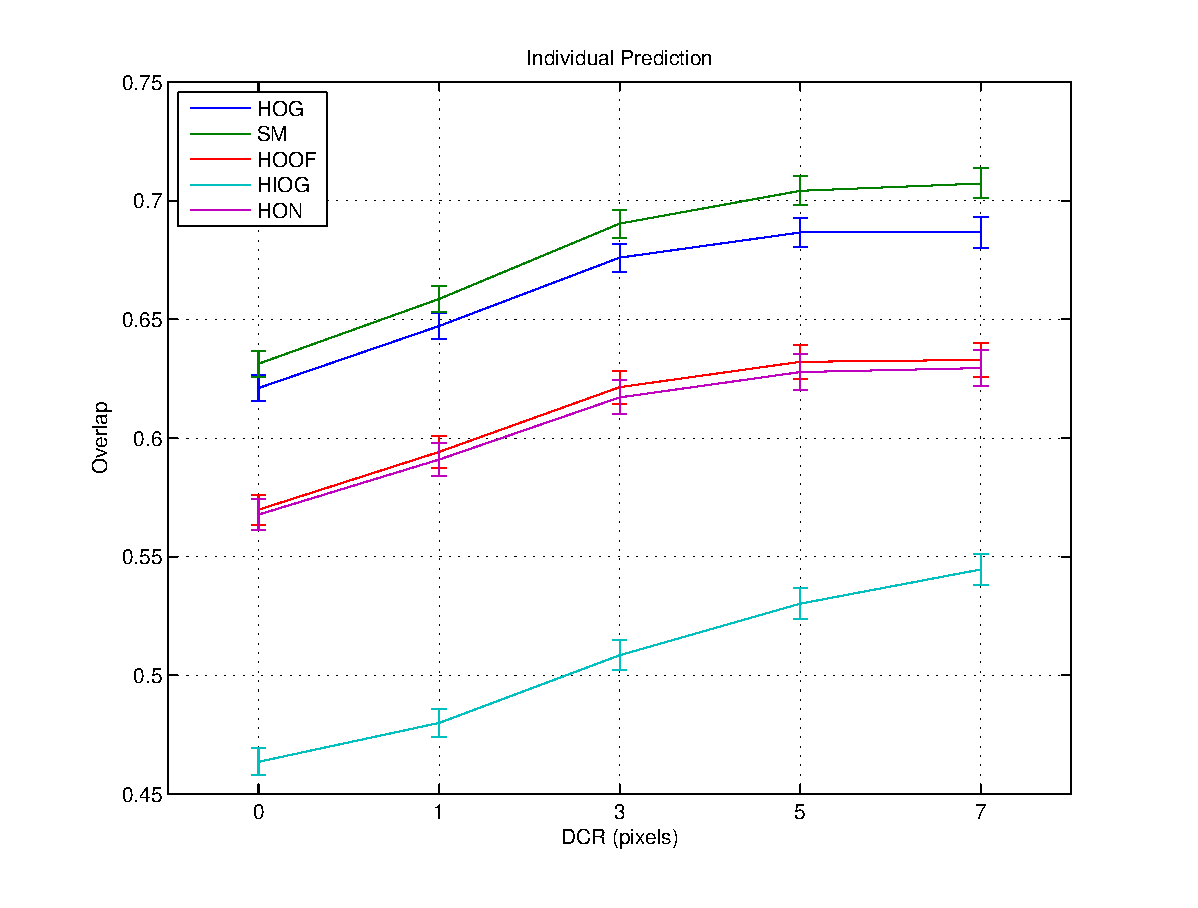
\includegraphics[width=1\textwidth]{results/individualprediction.eps}
 		\caption{Individual prediction}
    		\label{fig:individualprediction}
 	\end{subfigure}
	 ~
	\begin{subfigure}[b]{0.47\textwidth}
 		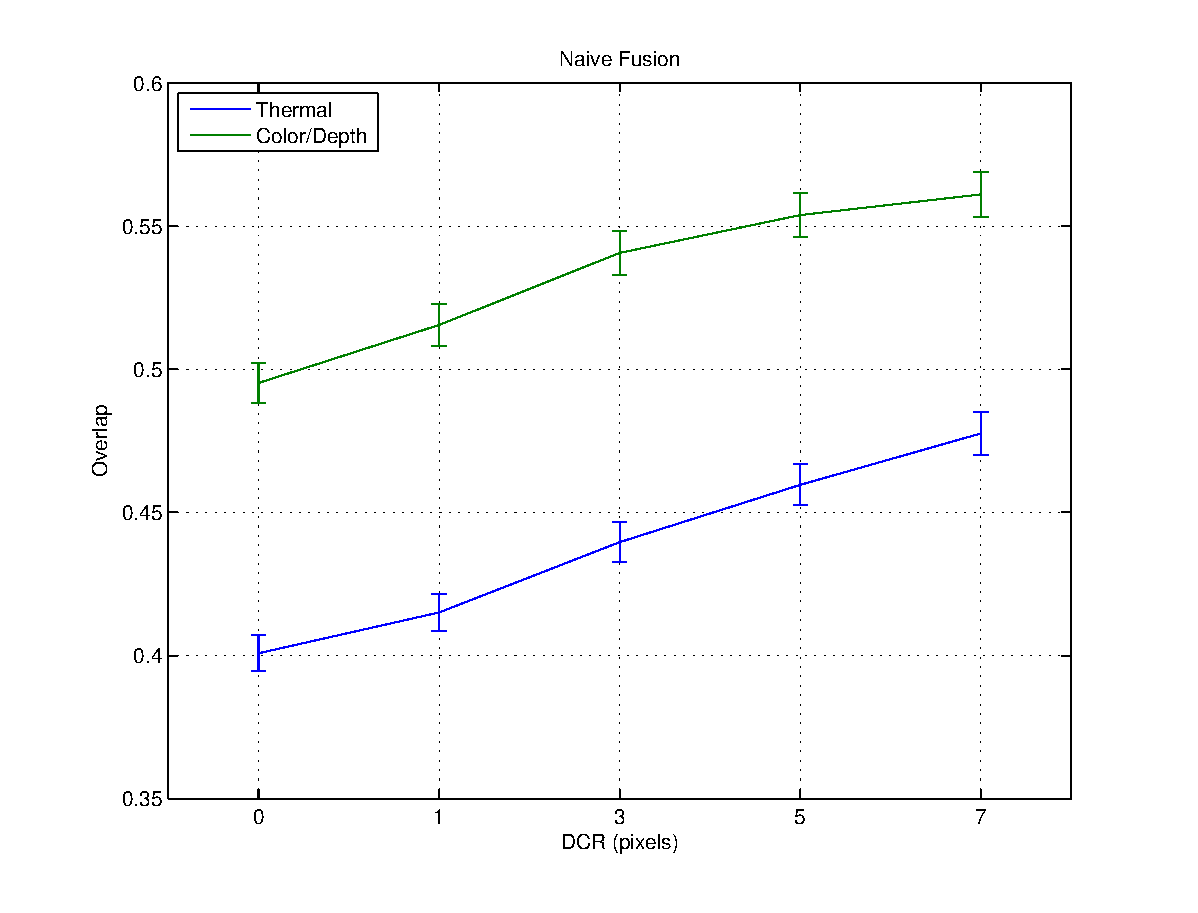
\includegraphics[width=1\textwidth]{results/naivefusion.eps}
 		\caption{Naive fusion}
    		\label{fig:naivefusion}
 	\end{subfigure}
	 \\
	\begin{subfigure}[b]{0.47\textwidth}
 		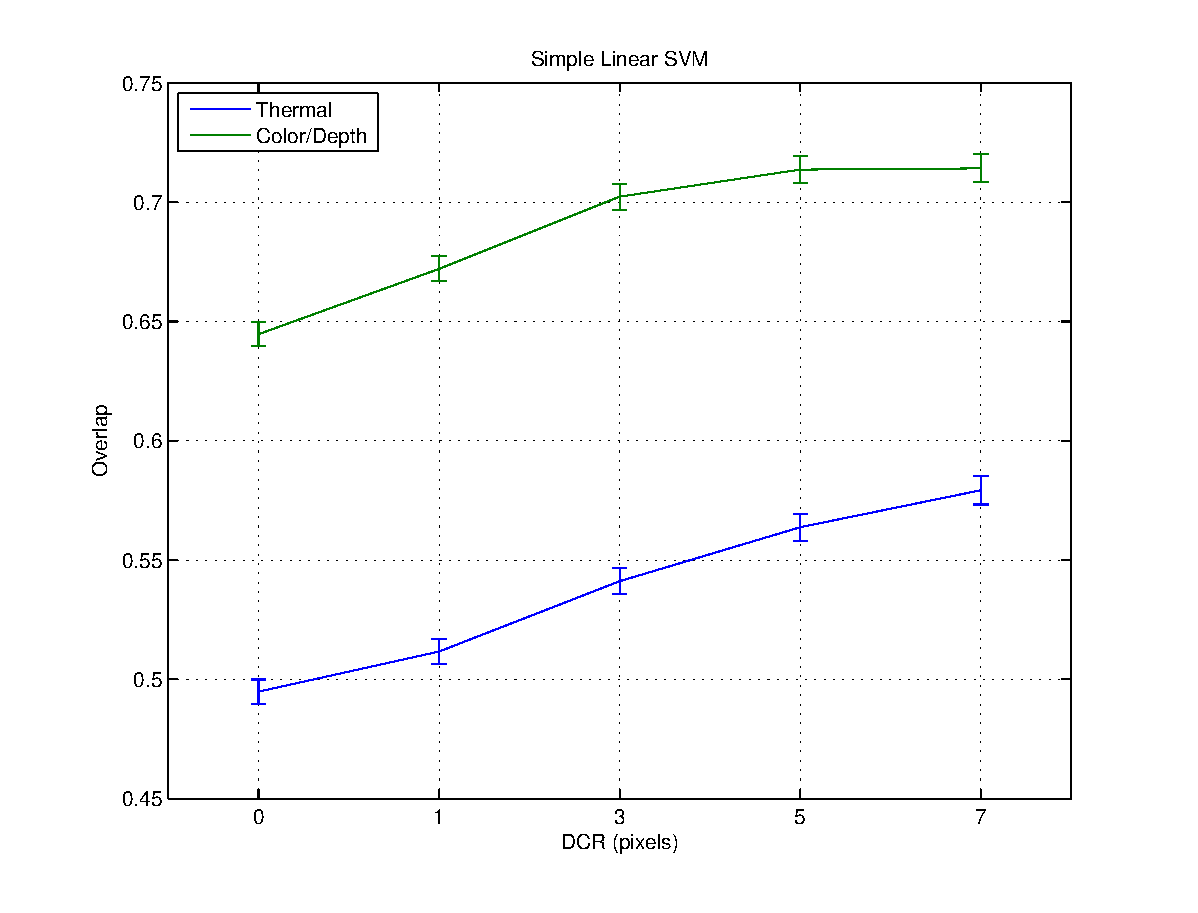
\includegraphics[width=1\textwidth]{results/simplelinearsvm.eps} 			
		\caption{Fusion using Simple linear SVM}
    		\label{fig:simplelinearsvm}
 	\end{subfigure}
	~
	\begin{subfigure}[b]{0.47\textwidth}
 		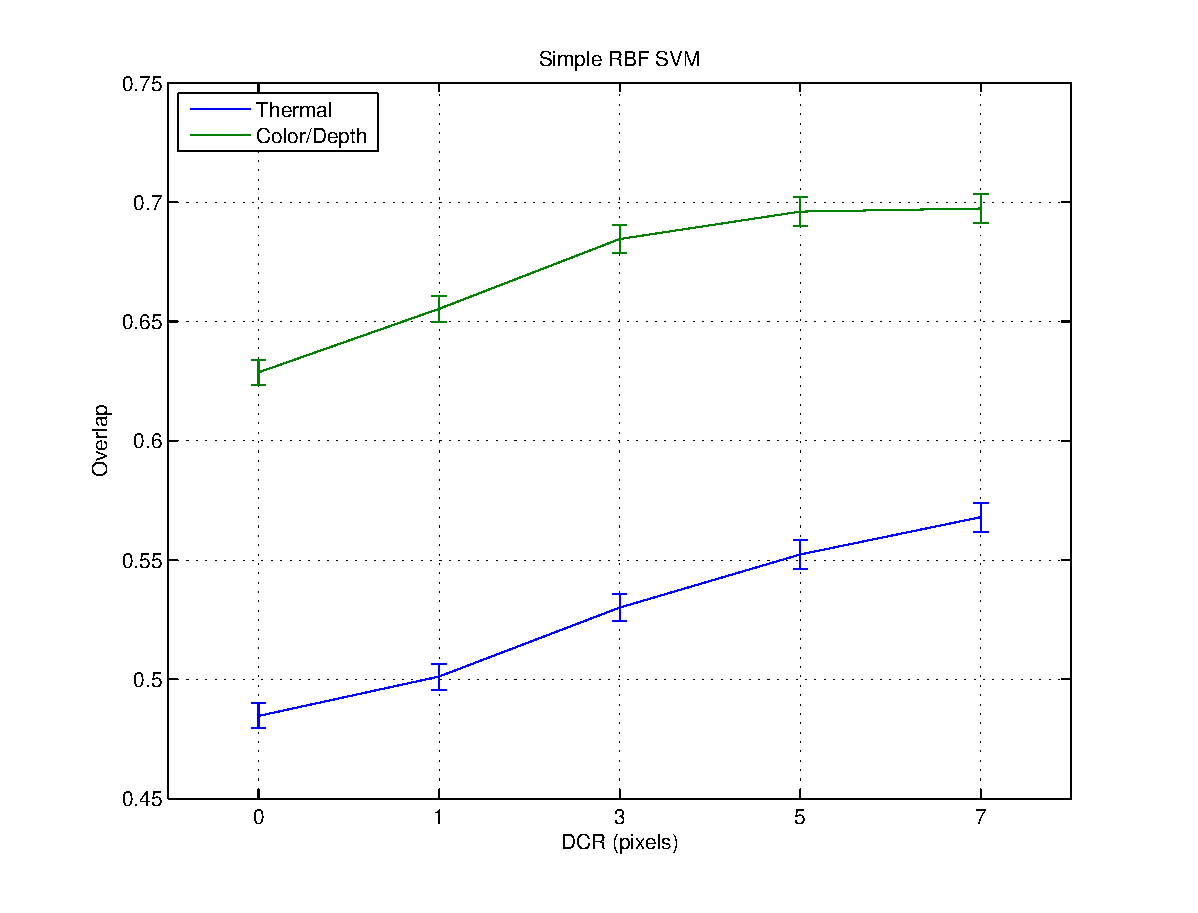
\includegraphics[width=1\textwidth]{results/simplerbfsvm.eps} 			
		\caption{Fusion using Simple RBF SVM}
    		\label{fig:simplerbfsvm}
 	\end{subfigure}
	\\
	\begin{subfigure}[b]{0.47\textwidth}
 		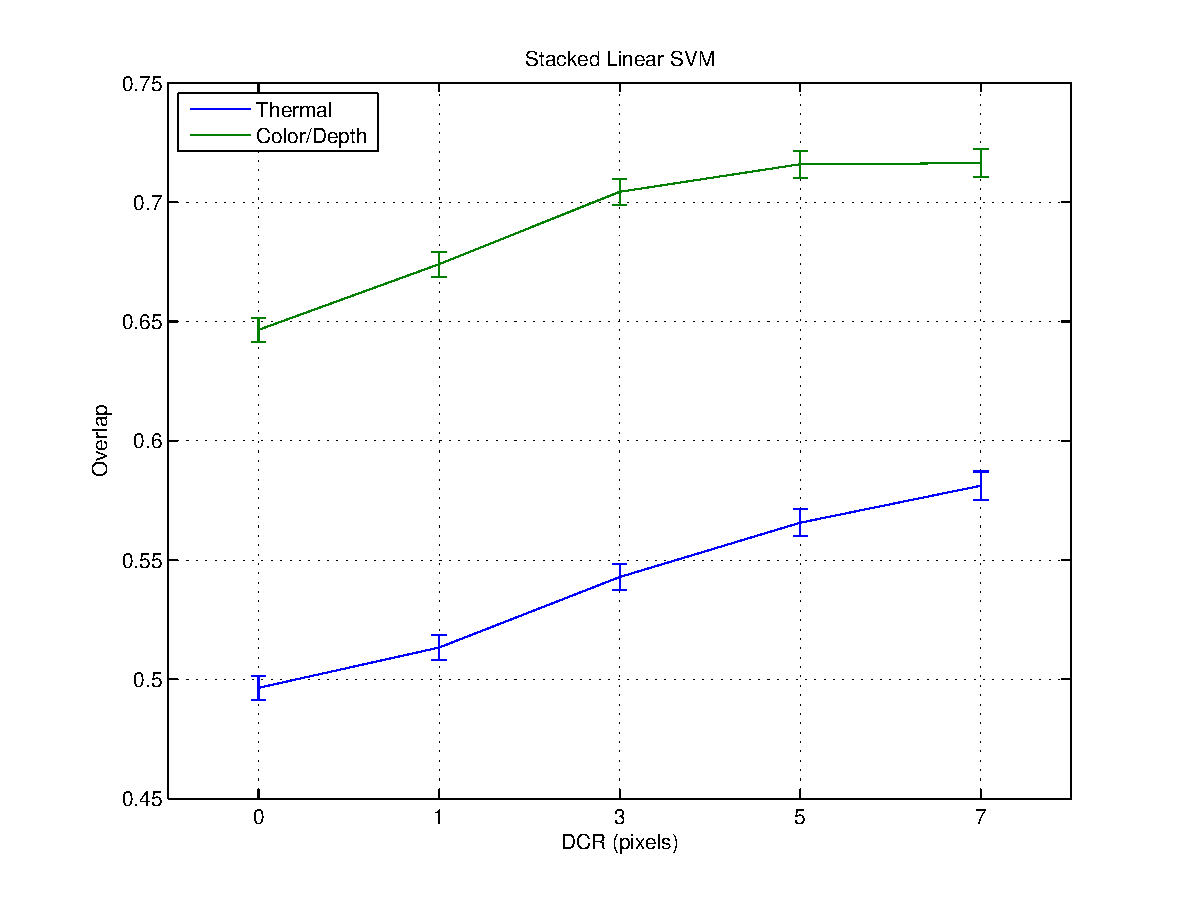
\includegraphics[width=1\textwidth]{results/stackedlinearsvm.eps} 			
		\caption{Fusion using Stacked Linear SVM}
    		\label{fig:stackedlinearsvm}
 	\end{subfigure}
	~
	\begin{subfigure}[b]{0.47\textwidth}
 		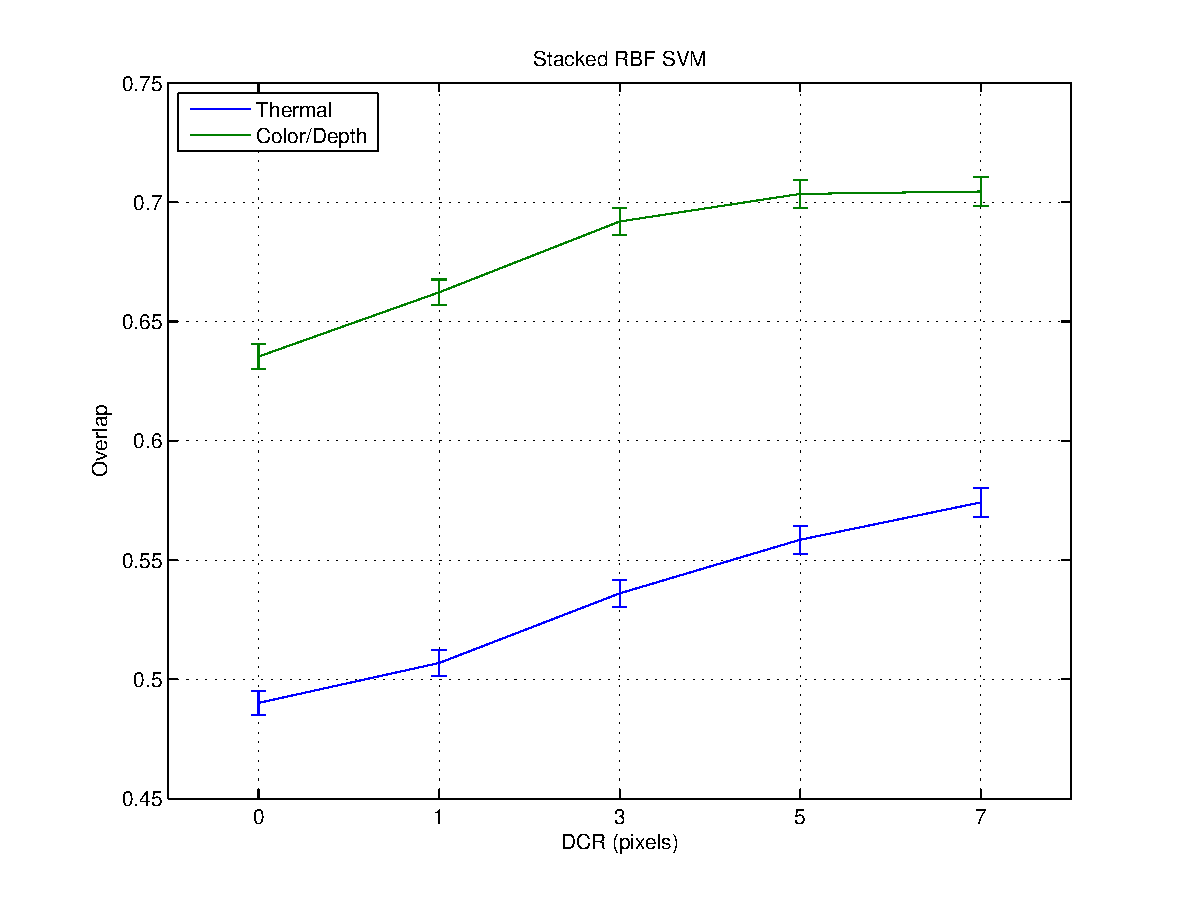
\includegraphics[width=1\textwidth]{results/stackedrbfsvm.eps} 			
		\caption{Fusion using Stacked RBF SVM}
    		\label{fig:stackedrbfsvm}
 	\end{subfigure}
	\caption{Overlap results for the different individual and fusion prediction approaches.}
	\label{fig:overlapgraph}
\end{figure}

\subsection{Discussion}
\label{ssec:discussion}

%add more comments
Furthermore, an upward trend is observed as the \emph{don't care region} (DCR) grows, although at higher DCR levels it stabilizes. This is comprehensible because usually the contours of the predicted masks are not accurately defined. Indeed, an accurate pixel-level segmentation is a rather complex task in state of the art techniques.

Having analyzed the experimental results, it is worth investigating the causes of some
misclassifications. One of the problems is originated in the beginning of the chain. Since
background subtraction reduces the search space, it may reject some actual person parts.
That mainly happens when a person is in the same depth than something which belongs
to the background model. Another issue is that some regions considered as unknown
mostly those generated when one person overlaps other considerably differ from those
that are used to train the different models. Consequently, the classification of such regions
is not a trivial task.

\section{Conclusions}
\label{sec:conclusions}
A solution for human body segmentation using a calibrated and registered multi-modal data has been proposed. Furthermore, a novel registered and annotated multi-modal RGB-Depth-Thermal data set of several video sequences has been introduced, which contains several
subjects interacting with everyday objects.

The first contribution of this work was an algorithm to register the different data modalities using multiple homographies generated from several views of the proposed calibration device. In addition, we presented a baseline for segmenting people which starts by an adaptive multi-modal background subtraction approach in order to extract the regions of interest that belong to a user or a moving object in the scene with high confidence. From the set of regions of interest coming
from the different data modalities, different state of the art descriptors have been used
and adapted to describe different feature vectors from each region. In particular, HOG and HOOF have been computed from RGB still images and image sequences, histogram of intensity gradients from thermal data, and histograms of normal vectors from depth maps coming from infrared sensors. The set of descriptors have been selected as the most discriminative ones given the results previously reported in literature.

Despite the obtained results, this proposal clearly leaves further room of improvement. To
begin with, the first background subtraction stage could combine the different modalities
in order to learn the model. Furthermore, a clustering of poses at cell-level could be
added before learning the GMMs. GrabCuts could also be applied to the predicted
segmentation binary masks to refine and smooth the contours, which would also produce
a rise in the segmentation accuracy.
{\small
\bibliographystyle{ieee}
\bibliography{references}
}

\end{document}
